%\documentclass[12pt]{report}
\documentclass[12pt, a4paper, oneside]{book}

% General imports:
\usepackage[utf8]{inputenc}
%\usepackage[utf8x]{inputenc} 
\usepackage[T1]{fontenc}	% For using icelandic Thorn character
\usepackage{amsmath}
\usepackage{amsfonts}		% Mathematic fonts (such Real numbers set)
\usepackage{graphicx}
\usepackage[spanish,es-tabla]{babel} 

% Imports for images
\usepackage{caption}
\usepackage{subcaption}
\usepackage{wrapfig}

% Imports for euro symbol support
\usepackage[official]{eurosym}
\DeclareUnicodeCharacter{20AC}{\euro{}}
%\newcommand{\euro}{€}

% Other imports:
\usepackage{indentfirst} % Indent first paragraph
\usepackage[colorlinks=false,pdfborder={0 0 0}]{hyperref}
%\usepackage[nottoc,numbib]{tocbibind} % Add bibliography to table of contents
\usepackage{url}
\hypersetup{urlcolor=black, colorlinks=false}
\usepackage{color}	% Color text


\usepackage{multirow, array} % para las tablas
\usepackage{float} % para usar [H]

% Formatting margins of the pages:
\usepackage[top=1.6cm, bottom=2.29cm, left=1.6cm, right=1.47cm]{geometry}

% Import for headersfig:estado_extrusora
\usepackage{fancyhdr}
\setlength{\headheight}{15pt}


\lhead{}
\chead{}
\rhead{}
\pagestyle{empty}


% Definitions of important data
\renewcommand{\author}{Santiago López Pina}
\renewcommand{\title}{SCADA Y MODELADO PARCIAL DE SISTEMA DE EXTRUSIÓN DE FILAMENTO}
\newcommand{\department}{Departamento de Sistemas y Automática}
\newcommand{\teacher}{Victor Gonzalez Pacheco}

%% All this is used for inserting C++ code on some parts of the thesis
\usepackage{listings}
\usepackage{color}

\definecolor{dkgreen}{rgb}{0,0.6,0}
\definecolor{gray}{rgb}{0.5,0.5,0.5}
\definecolor{mauve}{rgb}{0.58,0,0.82}


% This is for writing algorithms on pseudocode (nicely)
\usepackage{algorithm}
\usepackage[noend]{algpseudocode}

% Each chapter will have its own header
%\newcommand{\headchapter}[1]{\chapter{#1}\rhead{#1}}

% Each section will have its own header
%\newcommand{\headsection}[1]{\section{#1}}\rhead{#1}}

% Change 'Chapter' to something more logical
%\renewcommand{\chaptername}{}

% Define a command for comments
\newcommand{\comment}[1]{\textbf{\color{red} #1}}


% Define commands for setting the language to be used in listings
\newcommand{\Cpp}{ \lstset{frame=single,
  		language=C++,
  		aboveskip=3mm,
  		belowskip=3mm,
  		showstringspaces=false,
  		columns=flexible,
  		basicstyle={\small\ttfamily},
  		numbers=none,
  		numberstyle=\tiny\color{gray},
  		keywordstyle=\color{blue},
  		commentstyle=\color{dkgreen},
  		stringstyle=\color{mauve},
  		breaklines=true,
  		breakatwhitespace=true
  		tabsize=3
	}}


\newcommand{\XML}{
	\lstset{ language=XML, 
		morekeywords={ModularRobot, name, simulationFile, gaitTableFolder, frequencyTable, frequencyTable,
		 Module, Joint, Connections, front, left, right, back, connectedTo, connector, orientation, 
		 Orientation, Roll, Pitch, Yaw, serialPort}}}

\newcommand{\Bash}{
	\lstset{language=bash, morekeywords={mkdir, ls, make, sudo, apt-get, add-apt-repository, python}}}

%Full reference of label
\newcommand{\fullref}[1]{\ref{#1} de la página \pageref{#1}}
% This is used for adding appendices:	
\usepackage[toc,page]{appendix}

% This is used for tables spanning more than one page:
\usepackage{longtable}
	
% This is for units not appearing as italics
\usepackage{siunitx}
		
% This is for including pdf files
\usepackage{pdfpages}

% Enable hyphenation
\usepackage{hyphenat}

% Include PDF files
\usepackage{pdfpages}

%%%% BEGIN DOCUMENT %%%%%%%%%%%%%%%%%%%%%%%%%%%%%%%%%%%%%%%%%%%%%%%%%%%%%%%%%%%%%%%%
\begin{document}

%%%% FRONTPAGE %%%%%%%%%%%%%%%%%%%%%%%%%%%%%%%%%%%%%%%%%%%%%%%%%%%%%%%%%%%%%%%%
%\begin{center}
	
\includegraphics[width=0.25\textwidth]{./images/Logo.jpg}\\[2cm]
	\textsc{\LARGE Universidad Carlos III de Madrid}\\[0.5cm]
	\textsc{\LARGE \department}\\[0.5cm]
	\textsc{Grado en Ingeniería Electrónica, Industrial y Automática}\\[3cm]
	\textsc{\huge Trabajo final de grado}\\[1cm]
	\textsc{\LARGE \title}\\[6cm]
	\begin{table}[!ht]
	\centering
		\begin{tabular}{l l}
			Alumno: & \author \\
			Tutor: & \teacher\\
		\end{tabular}
	\end{table}

\end{center}
%====================================%
\pagestyle{plain}

%%%%%%Table of contents %%%%%%%%%%%%%%%%%%%%%%%%%%%%%%%%%%%%%%%%%%%%%%%%%%%%%%%%%%%%%
\tableofcontents
\newpage

% Figures
\listoffigures
% Tables
\listoftables




% Adding some header text on top of the page:
\fancyhead[L]{\nouppercase{\leftmark}}
\fancyhead[RO]{\nouppercase{\rightmark}}
\fancyhead[R]{}
\fancyhead[LO]{}
\pagestyle{fancy}

% Secciones del documento

\chapter{Estado del arte}
\label{cap:estado}
A la hora de tener una supervisión sobre la información producida a lo largo de un proceso productivo y poder tratarla a posteriorí, se usan sistemas software capaces de recopilar la información requerida en tiempo real del sistema y almacenarla para poder acceder a ella en un futuro.\\

Gracias a la informatización de la industria, estos sistemas están muy integrados dentro del proceso productivo puesto que, además de recopilar la información, se puede tener control directo en la producción. Una de las ventajas derivadas de la informatización, es que para tener el control del proceso, no es necesario encontrarse en el mismo lugar del mismo, gracias a Internet, se puede acceder desde cualquier parte del mundo y con cualquier dispositivo.\\

La palabra SCADA se usa para abreviar el término en inglés Supervisory Control And Data Adquisition o lo que es lo mismo, control supervisado y adquisición de datos. Un sistema SCADA puede ser utilizado en cualquer tipo de proceso en el cual se genere una cierta información que deba ser tratada por alguna persona, y se encuentre en un lugar remoto de la localización del proceso. En la Figura \ref{fig:smart_Controls} podemos observar un ejemplo de sistema SCADA orientado a la extrusión.\\

\begin{figure}[h!]
    \centering
    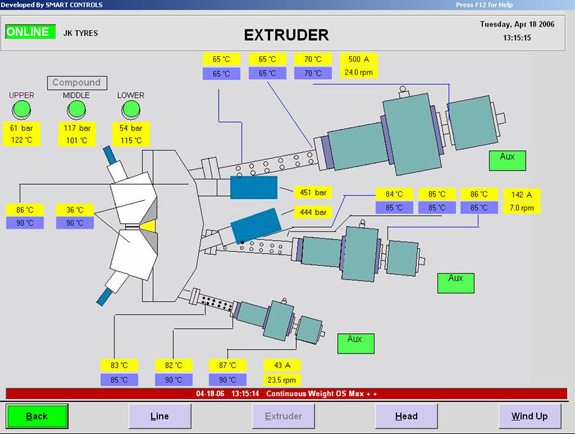
\includegraphics[width=0.6\textwidth]{images/triplex-extruder.jpg}
    \caption[Solución SCADA de la empresa SmartControls.]{Solución SCADA de la empresa SmartControls. Podemos apreciar como desde el sistema SCADA se accede a todas las variables que intervienen en el sistema. Fuente \cite{smartcontrols}.}
    \label{fig:smart_Controls}
\end{figure}

En lo referente a este tipo de aplicaciones, se han realizado avances y empresas como: Siemens, Wonderware, ABB o Rockwell Automation, ofrencen soluciones para implementar un sistema SCADA, y a día de hoy, prácticamente las soluciones son compatibles unas con otras.\\

Las distintas funciones que debe proveer un sistema SCADA son:

\begin{itemize}
    \item{Adquisición en tiempo real de los datos de intereses.}
    \item{Posibilidad de realizar gráficas de los datos adquiridos.}
    \item{Análisis de los datos obtenidos.}
    \item{Control sobre los distintos instrumentos del sistema.}
    \item{Acceso remoto al proceso productivo.}
\end{itemize}

Debido a la versatilidad de un sistema SCADA, son pocas las empresas que se dedican a una rama en concreto, se suele trabajar bajo pedido, y se diseñan sistemas SCADAS especificos para cada caso, sin embargo empresas como Castool ofrecen soluciones sistemas SCADA capaces de controlar totalmente el proceso productivo de la extrusión, Visual Optimizer \cite{castool}.\\

Castool ofrece un sistema de extrusión completo, suministrando tanto la maquinaría, software como personal cualificado para el uso de la máquina. Sin embargo esta solución solo sería útil en el caso que se adquiriera una línea de extrusión completa, en la mayoría de los casos no es lo habitual, puesto que siempre se suelen tener elementos de la linea de distintos fabricantes.\\







\chapter{Introducción y objetivos}
\label{cap:introduccion}

En la actualidad, la empresa BQ se ha especializado en fabricar y distribuir impresoras 3D junto con sus consumibles. En 2013, se creó un departamento de Innovación y Desarrollo, encabezado por Juan Gonzalez y Alberto Valero. En ese comienzo se distribuye material relacionado con las impresoras 3D para que cualquier persona pueda hacerse una impresora 3D. Este material no es fabricado por BQ directamente, se hace la tarea distribuidor.\\

A medida que BQ adquiere experiencia en el mercado, empieza a crear una línea de investigación para desarrollar sus propias impresoras 3D, como es el caso de la impresora Witbox y la impresora Prusa Hephestos (ver figura \ref{fig:impresoras_bq}). En este casos BQ tiene un papel importante a lo largo del desarrollo del producto, desde la elección de las características finales del mismo, así como el aspecto final del packaging, es decir, BQ pasa de tener un papel de distribuidor a ser la parte principal del desarrollo del producto.\\

\begin{figure}[H]
    \centering
    \begin{subfigure}[b]{0.4\textwidth}
        \centering
        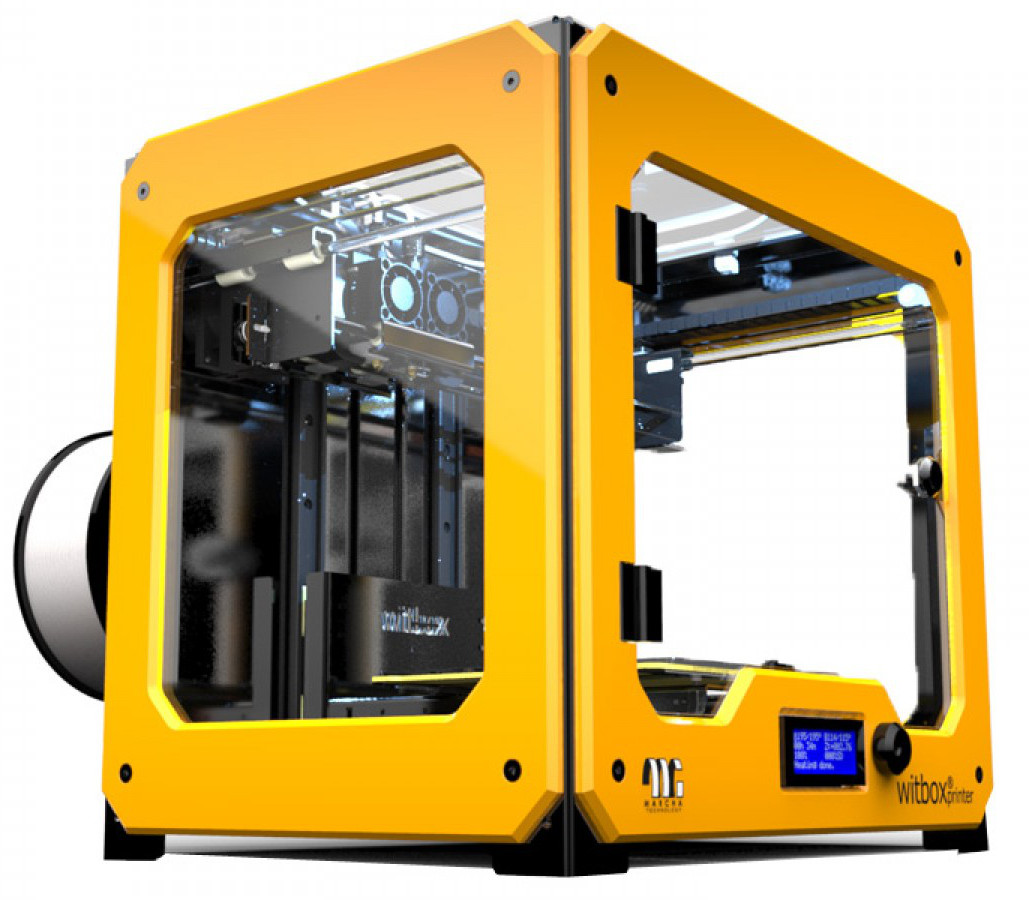
\includegraphics[width=\linewidth]{images/Witbox.jpg}
        \label{fig:estado_witbox}
    \end{subfigure}
    ~
    \begin{subfigure}[b]{0.3\textwidth}
        \centering
        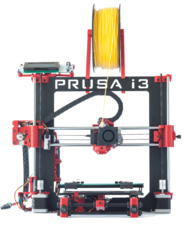
\includegraphics[width=\linewidth]{images/190px-HEPHESTOS.png}
        \label{fig:estado_hephestos}
    \end{subfigure}
    \caption[Impresoras fabricadas por BQ.]{Impresoras fabricadas por BQ. Podemos ver las dos impresoras que desarrolla BQ, a la izquierda, Witbox impresora que ya se vende montada. A la derecha, Prusa Hephestos, se vende en formato kit para que el usuario final la monte (DIY). Fuente \cite{bq}.}
    \label{fig:impresoras_bq}
\end{figure}

A la vez que se venden las impresoras 3D, BQ también vende el principal consumible para que las impresoras 3D puedan funcionar, plástico en forma de filamento. Este plástico se distribuye en unas bobinas (ver figura \ref{fig:estado_filamento}), en las que está almacenado un hilo continuo de plástico con un diámetro específico, en este caso, $1.75mm$, así mismo, cada filamento tiene un color distinto. Este consumible, es creado por otras empresas y BQ simplemente distribuye. Una vez que BQ tiene un puesto en el mercado de las impresoras 3D, decide entonces crear su propio filamento y tener más controlado la calidad del filamento que vende.\\

\begin{figure}[H]
    \centering
    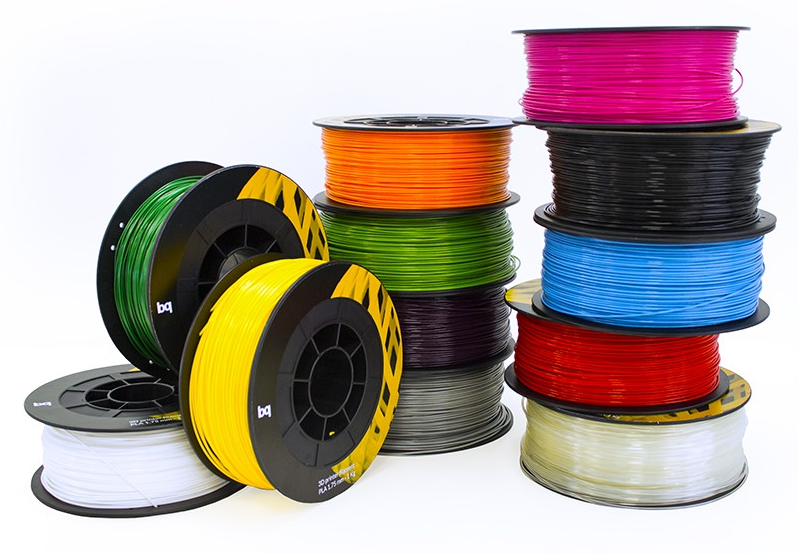
\includegraphics[width=0.5\textwidth]{images/filamento_bq.png}
    \caption[Distintos filamentos de BQ.]{Distintos filamentos de BQ. Fuente \cite{bq}}
    \label{fig:estado_filamento}
\end{figure}

Sin embargo, la fabricación del filamento es más complicada que la construcción de las impresoras 3D. Se necesitan máquinas capaces de fundir plástico y darle la forma de filamento, estás máquinas son las extrusoras, de las cuales BQ no dispone ninguna y no se tiene previsión de que al comprar una se pueda llegar a amortizar su compra. Por ello, se decide sub-contratar el proceso de fabricación a una empresa experta en la extrusión de plásticos.\\

En la provincia de Huesca, se encuentra la empresa PESL, la cual es especialista en extrusión de perfilería de plástico. BQ y PESL empiezan a trabajar en la fabricación de un filamento que cumpla las características necesarias para las impresoras 3D. En una primera aproximación estas características son, el material y el diámetro final. Después de pruebas de fabricación del filamento por parte de ambas empresas, BQ empieza a vender filamento propio.\\

Aparte de vender el filamento que fabrica PESL, BQ también lo usa para su uso en sus instalaciones y desarrollo de proyectos, se empieza a detectar entonces un problema, no todas las bobinas del mismo lote de fabricación tienen la misma calidad, llegando a darse el caso que en una misma bobina, no todo el filamento es igual. Los problemas detectados tienen que ver con el aspecto visual del filamento, la mezcla de color no es homogénea, y hace que las piezas impresas tenga un degradado. Así mismo, y mucho más importante, el diámetro del filamento no es constante (ver figura \ref{fig:muestra_filamento}).

\begin{figure}[H]
    \centering
    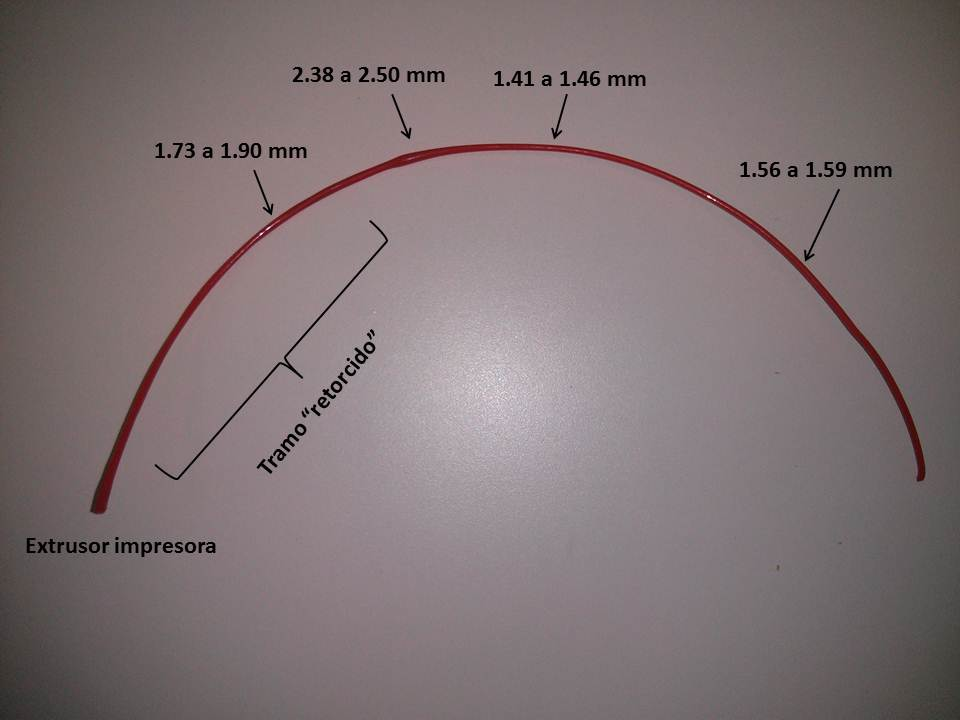
\includegraphics[width=0.6\textwidth]{images/atasco_rojo.jpg}
    \caption[Muestra de filamento con problemas en el diámetro]{Muestra de filamento con problemas en el diámetro. Podemos observar cómo en un tramo de filamento, el diámetro no es constante.}
    \label{fig:muestra_filamento}
\end{figure}

El problema que se tiene en el color, es algo secundario, ya que puede considerarse visual y no afecta a ninguno de los componentes de la impresora. No pasa lo mismo con el problema del diámetro, ya que la manera en la que se descubre, es que las impresoras dejan de imprimir pasado un tiempo, puesto que si el diámetro nominal del filamento sale de un determinado rango de valores, tanto por exceso como por déficit, se producen atascos en la impresora. Estos atascos, en el mejor de los casos, sólo supone la limpieza del extrusor de la impresora y se puede volver a utilizar, pero en ocasiones el atasco puede deja inservible el extrusor y es necesario reemplazarlo.\\

No tardan en llegar las primera reclamaciones de clientes finales, en las que su impresora deja de imprimir de forma temporal o incluso que el uso del filamento de BQ daña las impresoras 3D de los clientes, suponiendo un gasto extra para BQ, ya que ofrece una garantía por su producto y para PESL, que no todo el filamento que fabrica reporta beneficios. Es por ello que se pone en aviso a PESL y se toman decisiones para mejorar este problema.\\

A pesar de que PESL es especialista en extrusión de perfilería de plástico, es la primera vez que se dedican a la extrusión de filamento. Aunque de forma teórica no hay ninguna diferencia, si lo hay en el uso final que se va a dar al plástico. En el caso de un perfil extruido, su uso será rematar obras, recubrimiento aislante y tuberías. El uso final que se le va a dar al filamento de plástico va a suponer un refundido del material, proceso en el cual, influye la manera en cómo se fabricó. Igualmente el material con el que se trabaja, no es el mismo y requiere de otras condiciones de fabricación que las que se pensaba en una primera aproximación.\\ 

Se incorpora a la línea de fabricación un elemento mecánico, por el cual pasa el filamento, y si este supera un diámetro se parte y se deja de producir. También se empieza a registrar el diámetro del filamento y las temperaturas de fabricación en un ordenador para intentar tener un mejor control de la trazabilidad de las bobinas, y así acotar el problema que haya en la fabricación.\\

Las reclamaciones de los clientes siguen llegando a BQ y PESL y con ellas, las pérdidas para ambos. Gracias a que cada bobina contiene un código QR en el que se incluye el número de lote de fabricación, se solicitan los registros del lote de fabricación a PESL para intentar ver posibles causas. Sin embargo, el tiempo desde que se piden hasta que son dados, es demasiado amplio. Una vez que se tiene el registro, se comprueba que faltan datos de temperaturas, puesto que estos valores son introducidos a mano ya que no están conectados con el ordenador que registra la información del diámetro. Y el muestreo de los datos no es siempre constante, por lo que hay tramos de la bobina que no se tienen.\\

Desde BQ se decide entonces tomar una solución para tener todos los registros de una manera cómoda y fiable. Se piensa en desarrollar un sistema automático en el cual estén conectados todos los elementos que componen la línea de extrusión y así poder acceder a los datos de: Fecha de fabricación, diámetro final del filamento, temperaturas de todo el proceso y velocidad de extrusión. Así mismo, esta información será almacenada en una base de datos, la cual se podrá acceder de manera remota. De esta manera, se quita carga de trabajo a PESL para que se dediquen a fabricar filamento, y desde BQ se puedan analizar los datos para ver causas de fallo.\\

A continuación, se detallan los objetivos a conseguir en el proyecto:

\begin{itemize}
    \item Realizar un sistema capaz de leer la información más importante en la fabricación del filamento
    \item Instalar en una extrusora de filamento industrial.
    \item Estudio de los datos adquiridos y desarrollo del modelo teórico de la planta.
    \item Comprobar qué regulador se amolda a nuestras necesidades.
    \item Puesta en marcha del regulador en planta y comprobar resultados.
\end{itemize}
\label{Listado_objetivos}




\chapter{Objetivos}
\label{objetivos}

Como se ha comentado a lo largo del capítulo introductorio, para el correcto funcionamiento de la línea es necesario un operador que controle y supervise el funcionamiento de la misma, realice la carga de granza en la extrusora y la carga y descarga de los carretes en la bobinadora. Debido a ello se generan  errores en la producción que sólo son visibles una vez que el producto ha sido almacenado y es sometido a las convenientes pruebas de calidad, almacenando asi un producto que no es de la calidad necesaria para comercializarlo.\\

 Para minimizar el error humano, se propone la implementación de un sistema de aquisición y procesamiento de datos (SCADA) que permita el análisis durante y posterior la producción, de los diferentes parámetros del sistema. Con el fin de modelar parcialmente el mismo para tratar de cerrar el lazo de control entre la unidad tractora y el sistema de control del diámetro. De esta manera, podemos ver los aspectos que influyen en el diámetro y que el propio sistema sea capaz de corregirlo en tiempo real durante la producción.

El proyecto está definido por dos fases:\\

La primera fase en la que se desarrollará el sistema de adquisición de datos constará de los siguientes puntos:
\begin{itemize}
    \item Recopilación y análisis de la documentación de todos los dispositivos de interés para el proyecto de la línea de extrusión. Ya que actualmente disponemos de instrumentación que no hemos elegido nosotros, deberemos adquirir toda la documentación para poder lograr conseguir la automatización del sistema y ver cómo funciona individualmente cada uno.
    \item Defición de los requisitos respecto a comunicaciones necesarias entre los dispositivos de la línea y el sistema de adquisición.
    \item Determinar los requisitos del autómata progamable industrial (PLC) a utilizar.
    \item Programación del PLC. Puesto que será el encargado de llevar el control de la planta, deberemos programar la adquisición de datos, para establecer el control sobre la linea.
\end{itemize}

En esta fase, se pondrá en marcha todo el sistema en la planta, instalando el PLC y cableando toda la red de comunicaciones y sensores que disponemos. Así mismo se almacenarán datos de los seis sensores de temperatura que dispone la planta (cinco de ellos en extrusora y uno en bañera de enfriamiento), y sensor de diámetro. Con los datos adquiridos se modelará parcialmente la planta para intentar hacer un control en lazo cerrado entre la unión tractora de filamento y el sensor de diámetro del mismo. Durante esta fase se diseñará un sistema, para poder visualizar los datos adquiridos de forma remota.\\

La segunda fase del proyecto, consistirá en la implementación en planta de los distintos reguladores diseñados y probados en la fase anterior. Como primera aproximación la salida a controlar será el diámetro del filamento y la entrada la velocidad de extrusión, ya que es la variable que influye directamente en el diámetro a conseguir. Se estudiarán los beneficios de usar distintos tipos de controladores como pueden ser PID, fuzzy, etc. para posteriormente estudiar los beneficiós e inconvenientes de cada uno de ellos.\\

Para el completo desarrollo de esta segunda fase, y poder demostrar el correcto funcionamiento en la línea, necesitaremos la aprobación de la empresa que explota la línea de extrusión. Aunque se tratará de un sistema modular que será fácil de integrar en otras líneas de producción parecidas. Siendo el sistema totalmente compatible y escalable para futuras lineas de extrusión que se adquieran.\\

A continuación, se detallan los objetivos a conseguir en el proyecto y un diagrama de gant con la planificación inicial del proyecto:

\begin{itemize}
	\item Documentación de la instrumentación de la planta.
	\item Definir la arquitectura para la comunicación del PLC y la instumentación
	\item Definir requisitos del PLC a adquirir.
	\item Programación del PLC.
	\item Realización del armario eléctrico para montar en la fábrica.
	\item Estudio de los datos adquiridos y desarrollo del modelo teórico de la planta.
	\item Comprobar qué regulador se amolda a nuestras necesidades.
	\item Puesta en marcha del regulador en planta y comprobar resultados.
\end{itemize}


\chapter{Desarrollo}
\label{hardware}

\section{Búsqueda de información}
\label{busqueda_informacion}

El primer paso es identificar el hardware del que disponemo en la fábrica con ayuda de las fotos tomadas:
    \begin{figure}[H]
            \centering
            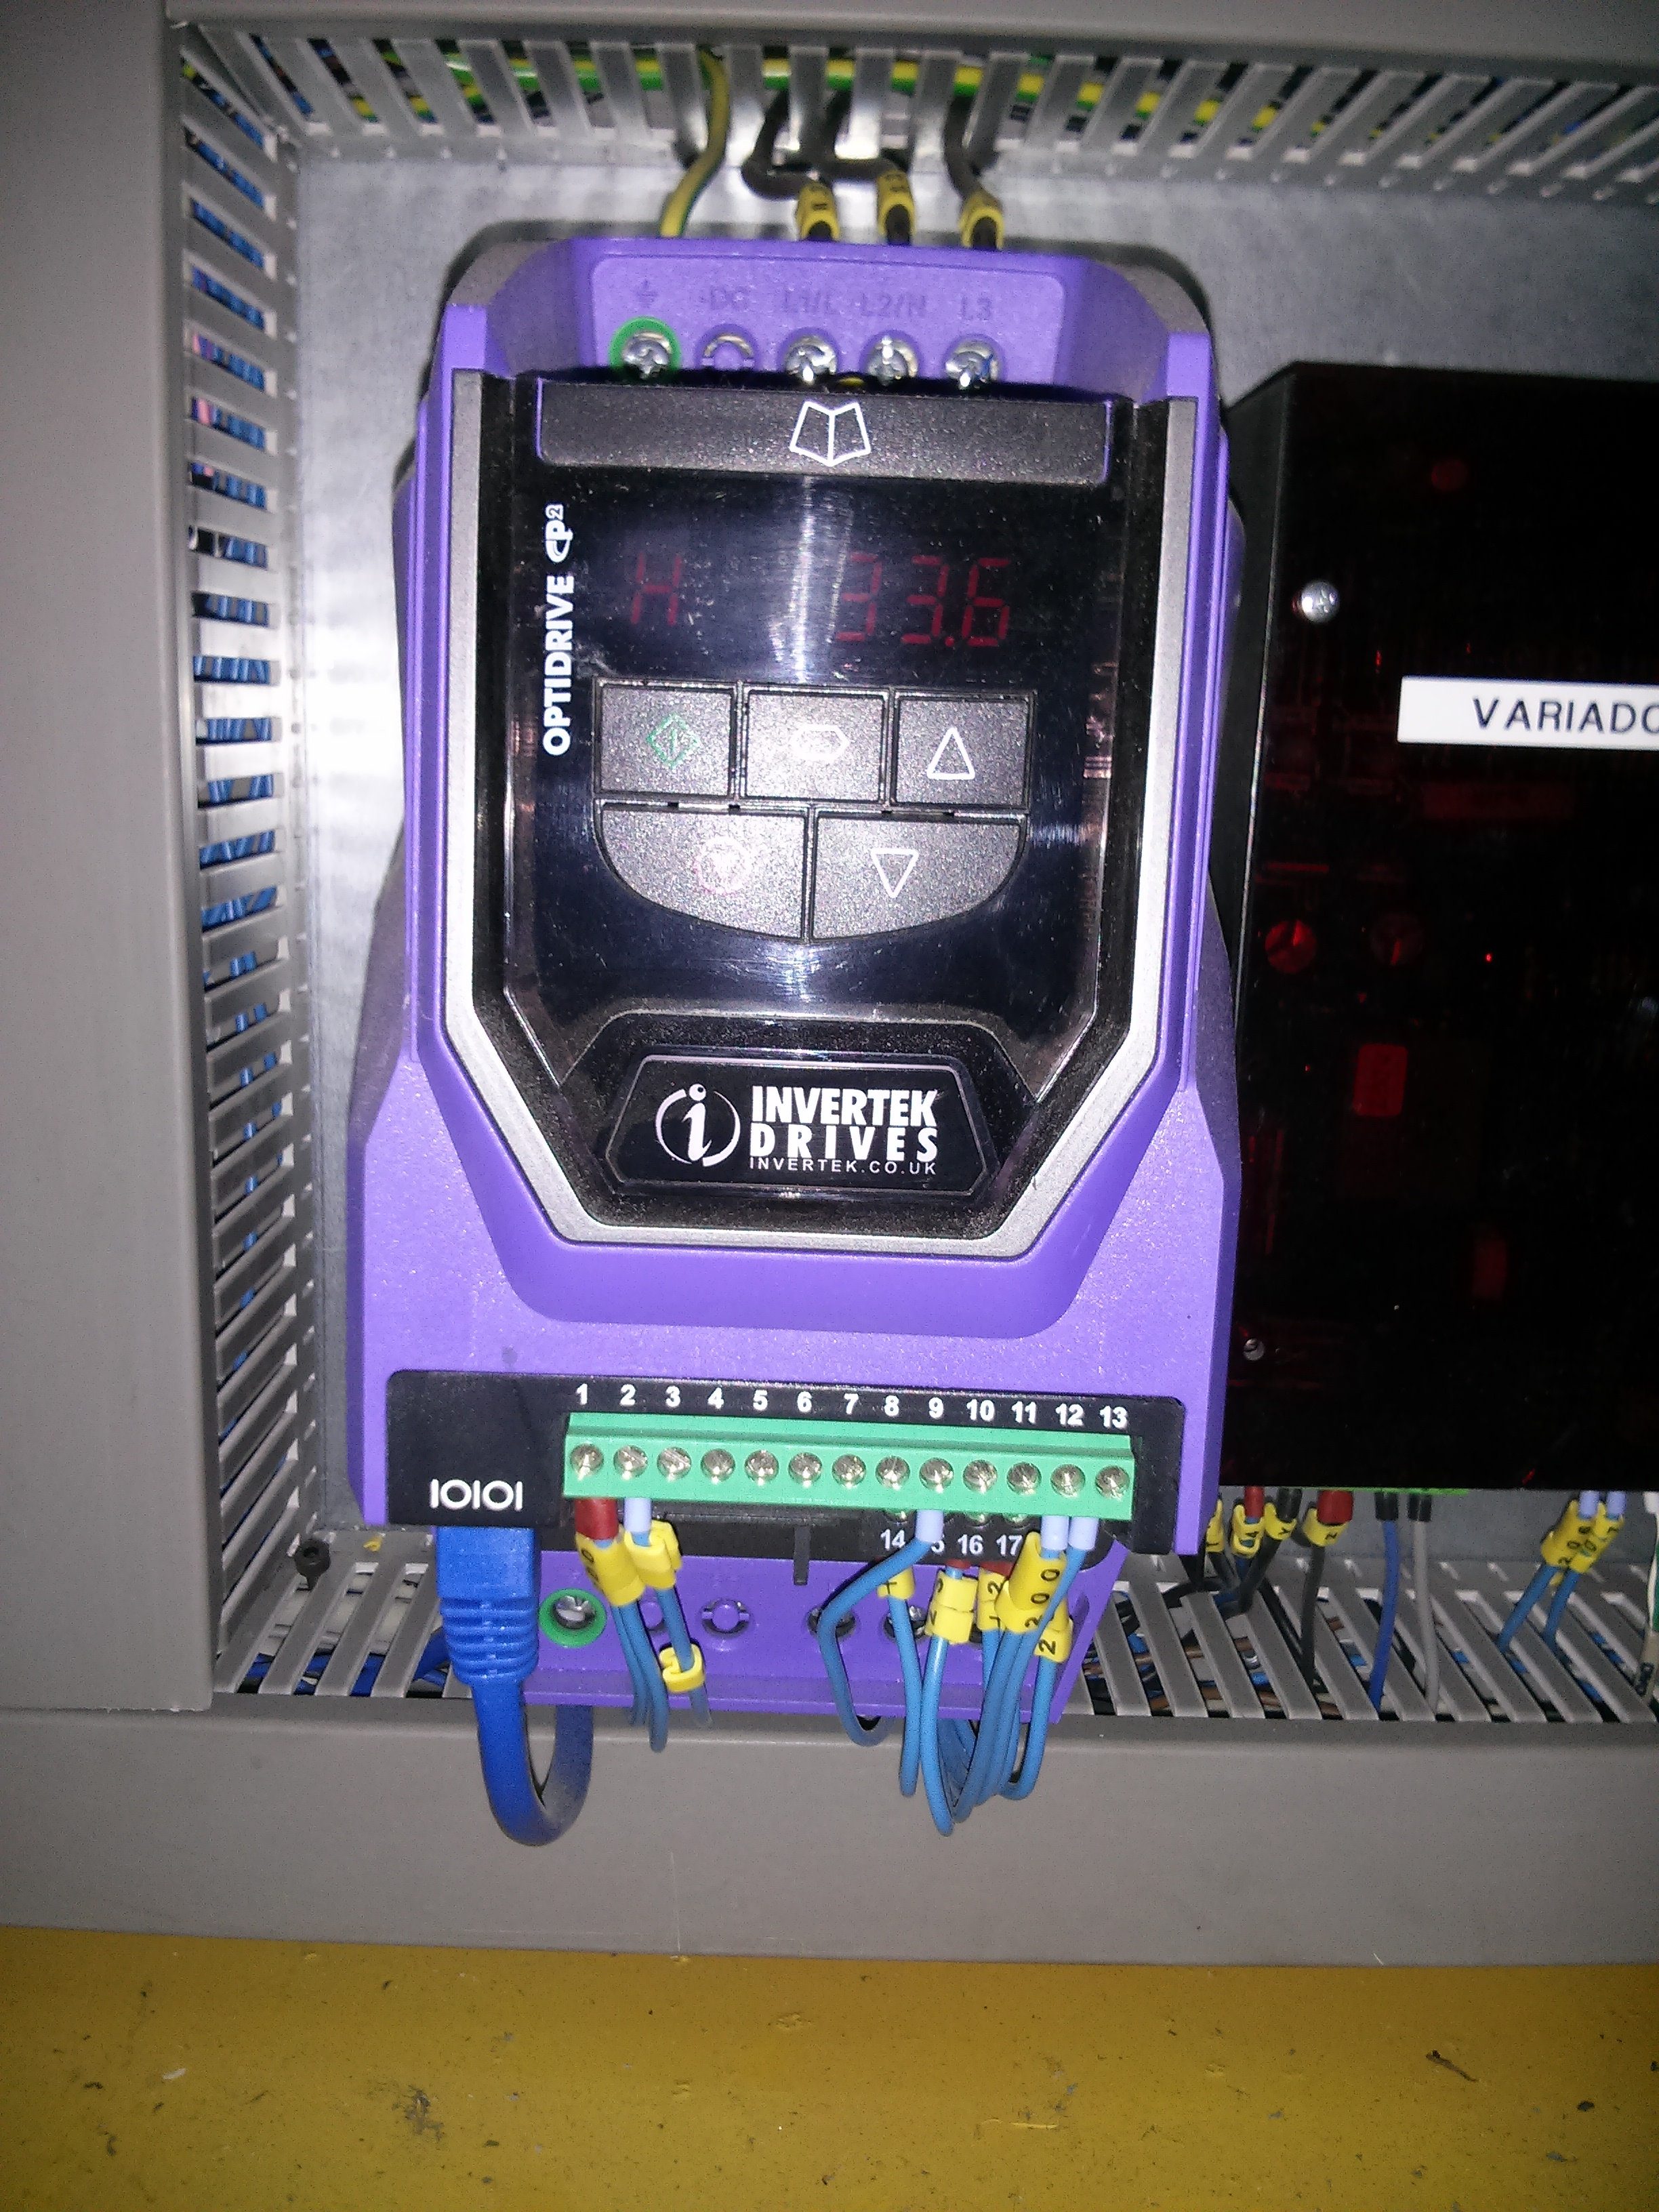
\includegraphics[width=0.4\textwidth]{images/huesca/IMG_20141216_174810.jpg}
            \caption{Variador Optidrive}
            \label{fig:hardware_variador}
    \end{figure}

    \begin{figure}[H]
            \centering
            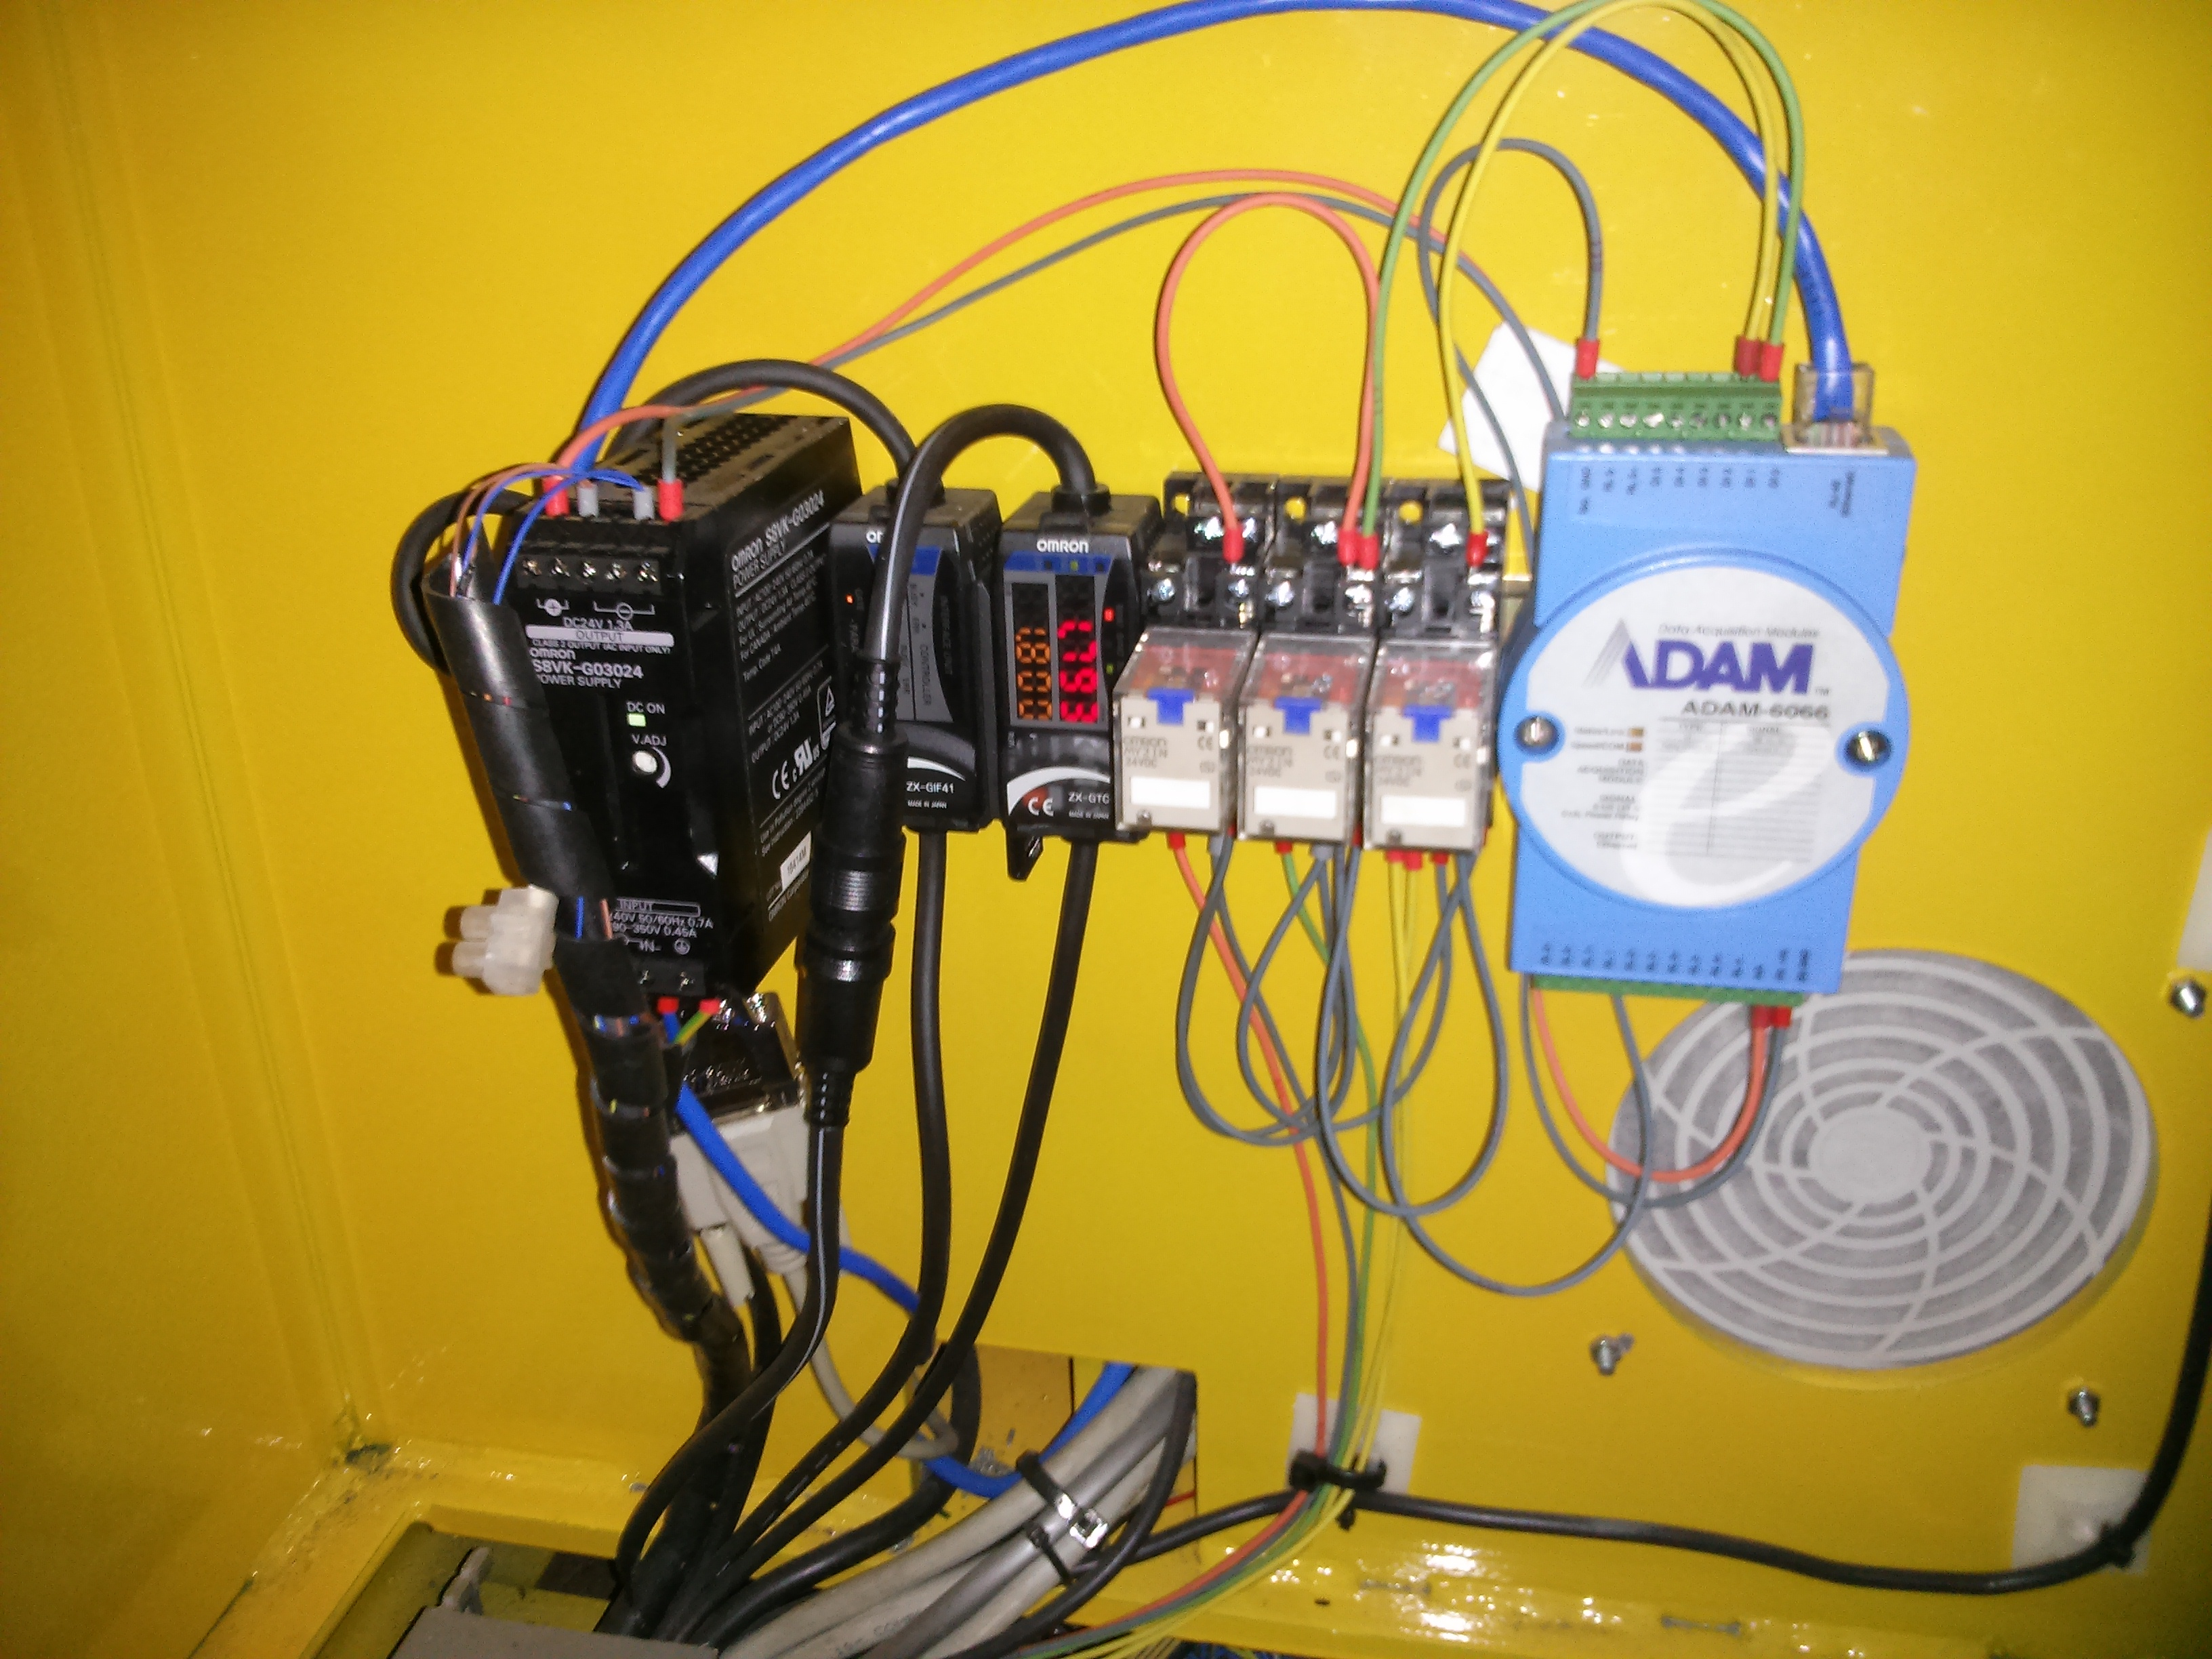
\includegraphics[width=0.4\textwidth]{images/huesca/IMG_20141216_174824.jpg}
            \caption{Sensor de diámetro y perifería}
            \label{fig:hardware_diametro}
    \end{figure}

    \begin{figure}[H]
            \centering
            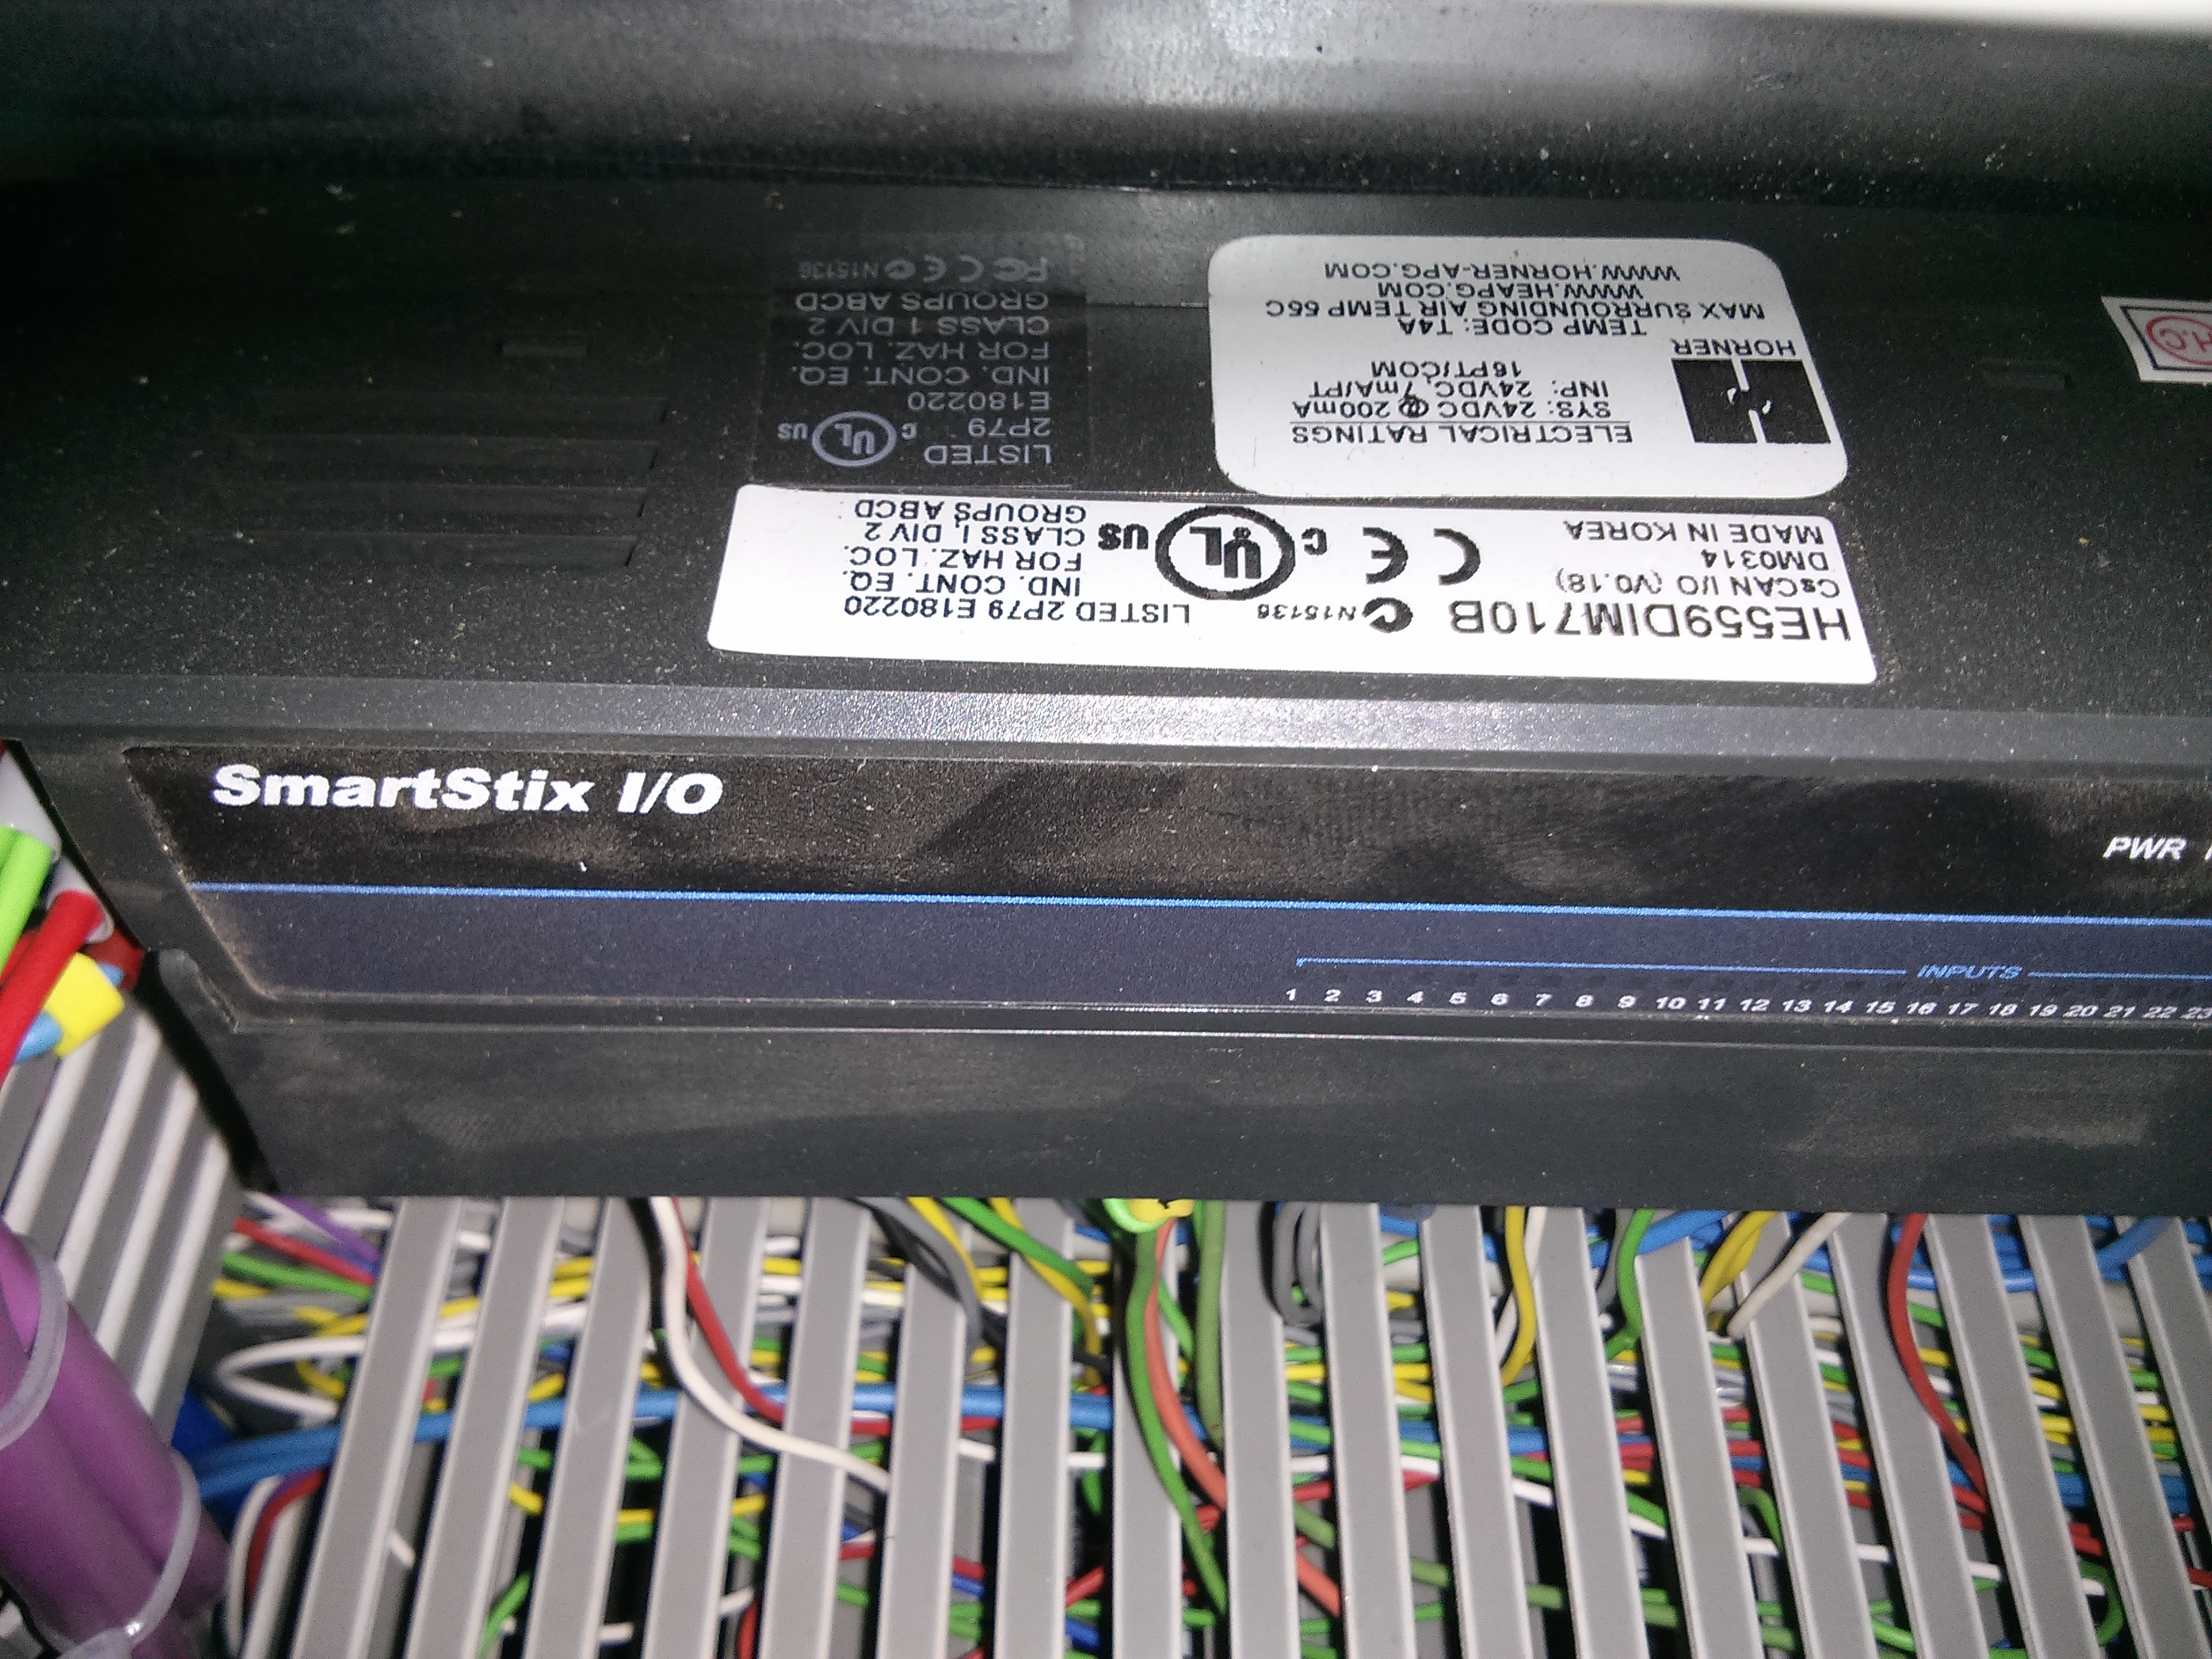
\includegraphics[width=0.4\textwidth]{images/huesca/IMG_20141216_174925.jpg}
            \caption{Perifería distribuida}
            \label{fig:hardware_periferia}
    \end{figure}

    \begin{figure}[H]
            \centering
            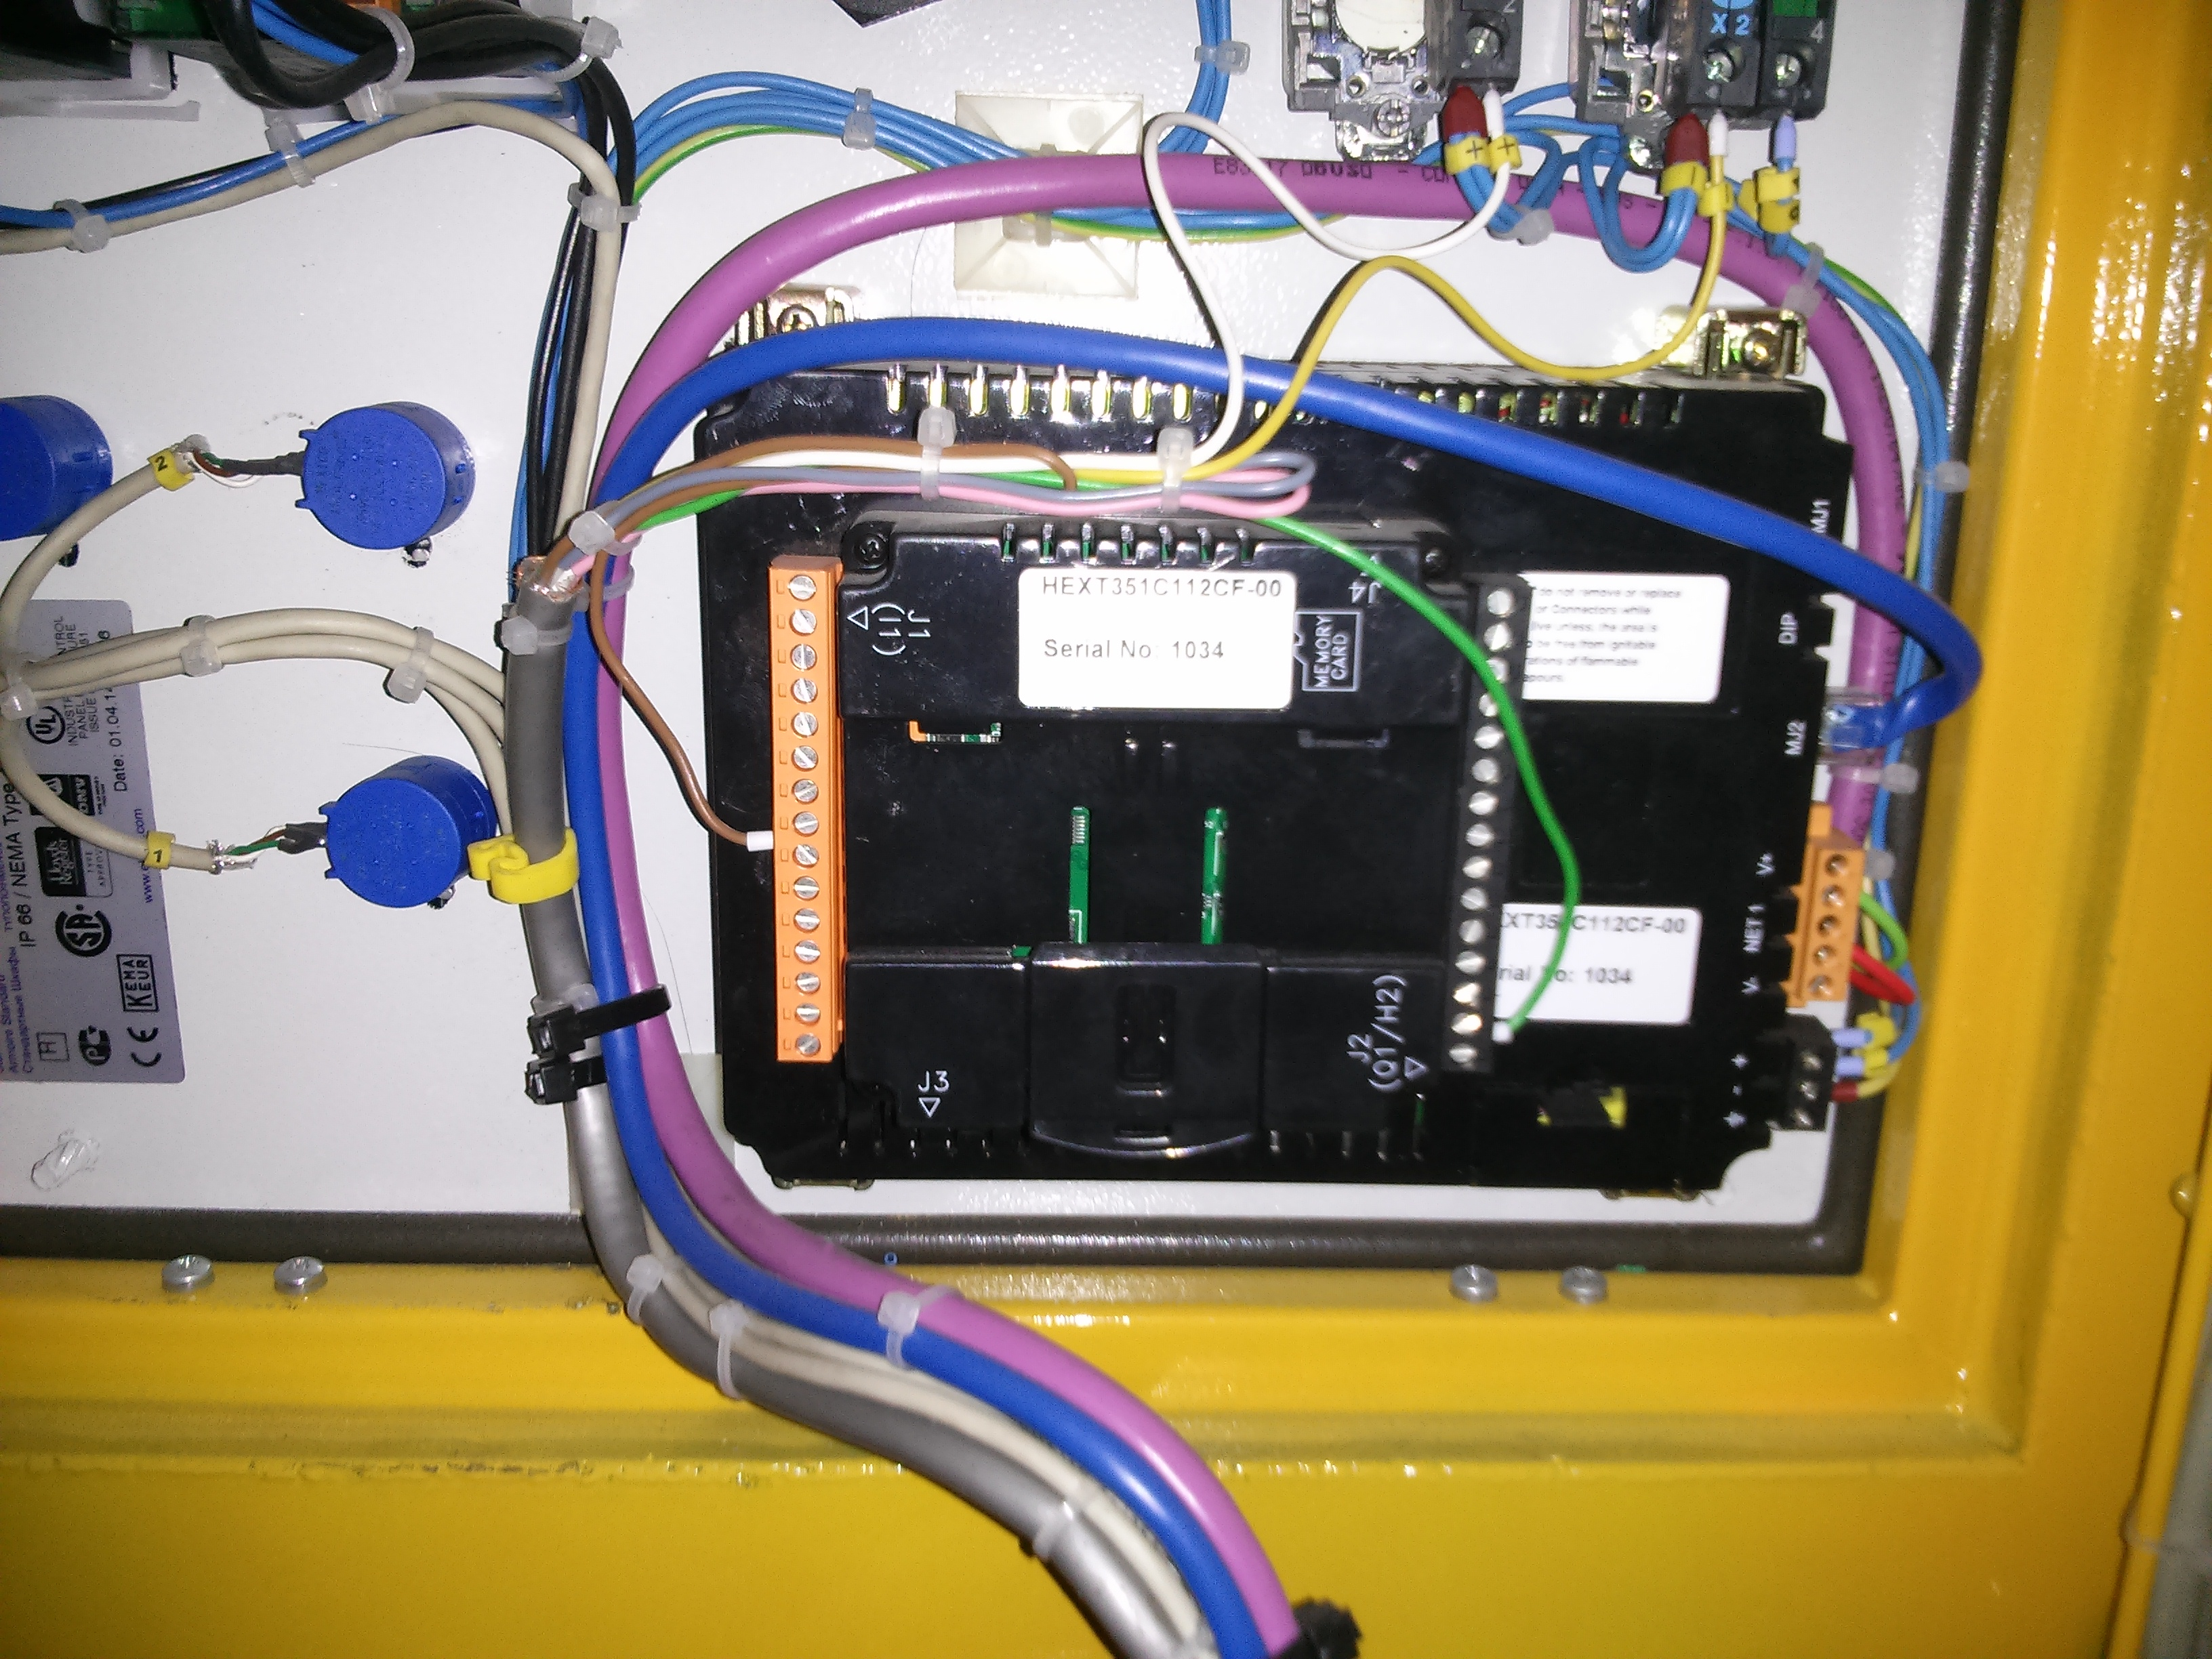
\includegraphics[width=0.4\textwidth]{images/huesca/IMG_20141216_175108.jpg}
            \caption{Pantalla HMI}
            \label{fig:hardware_HMI}
    \end{figure}

     \begin{figure}[H]
            \centering
            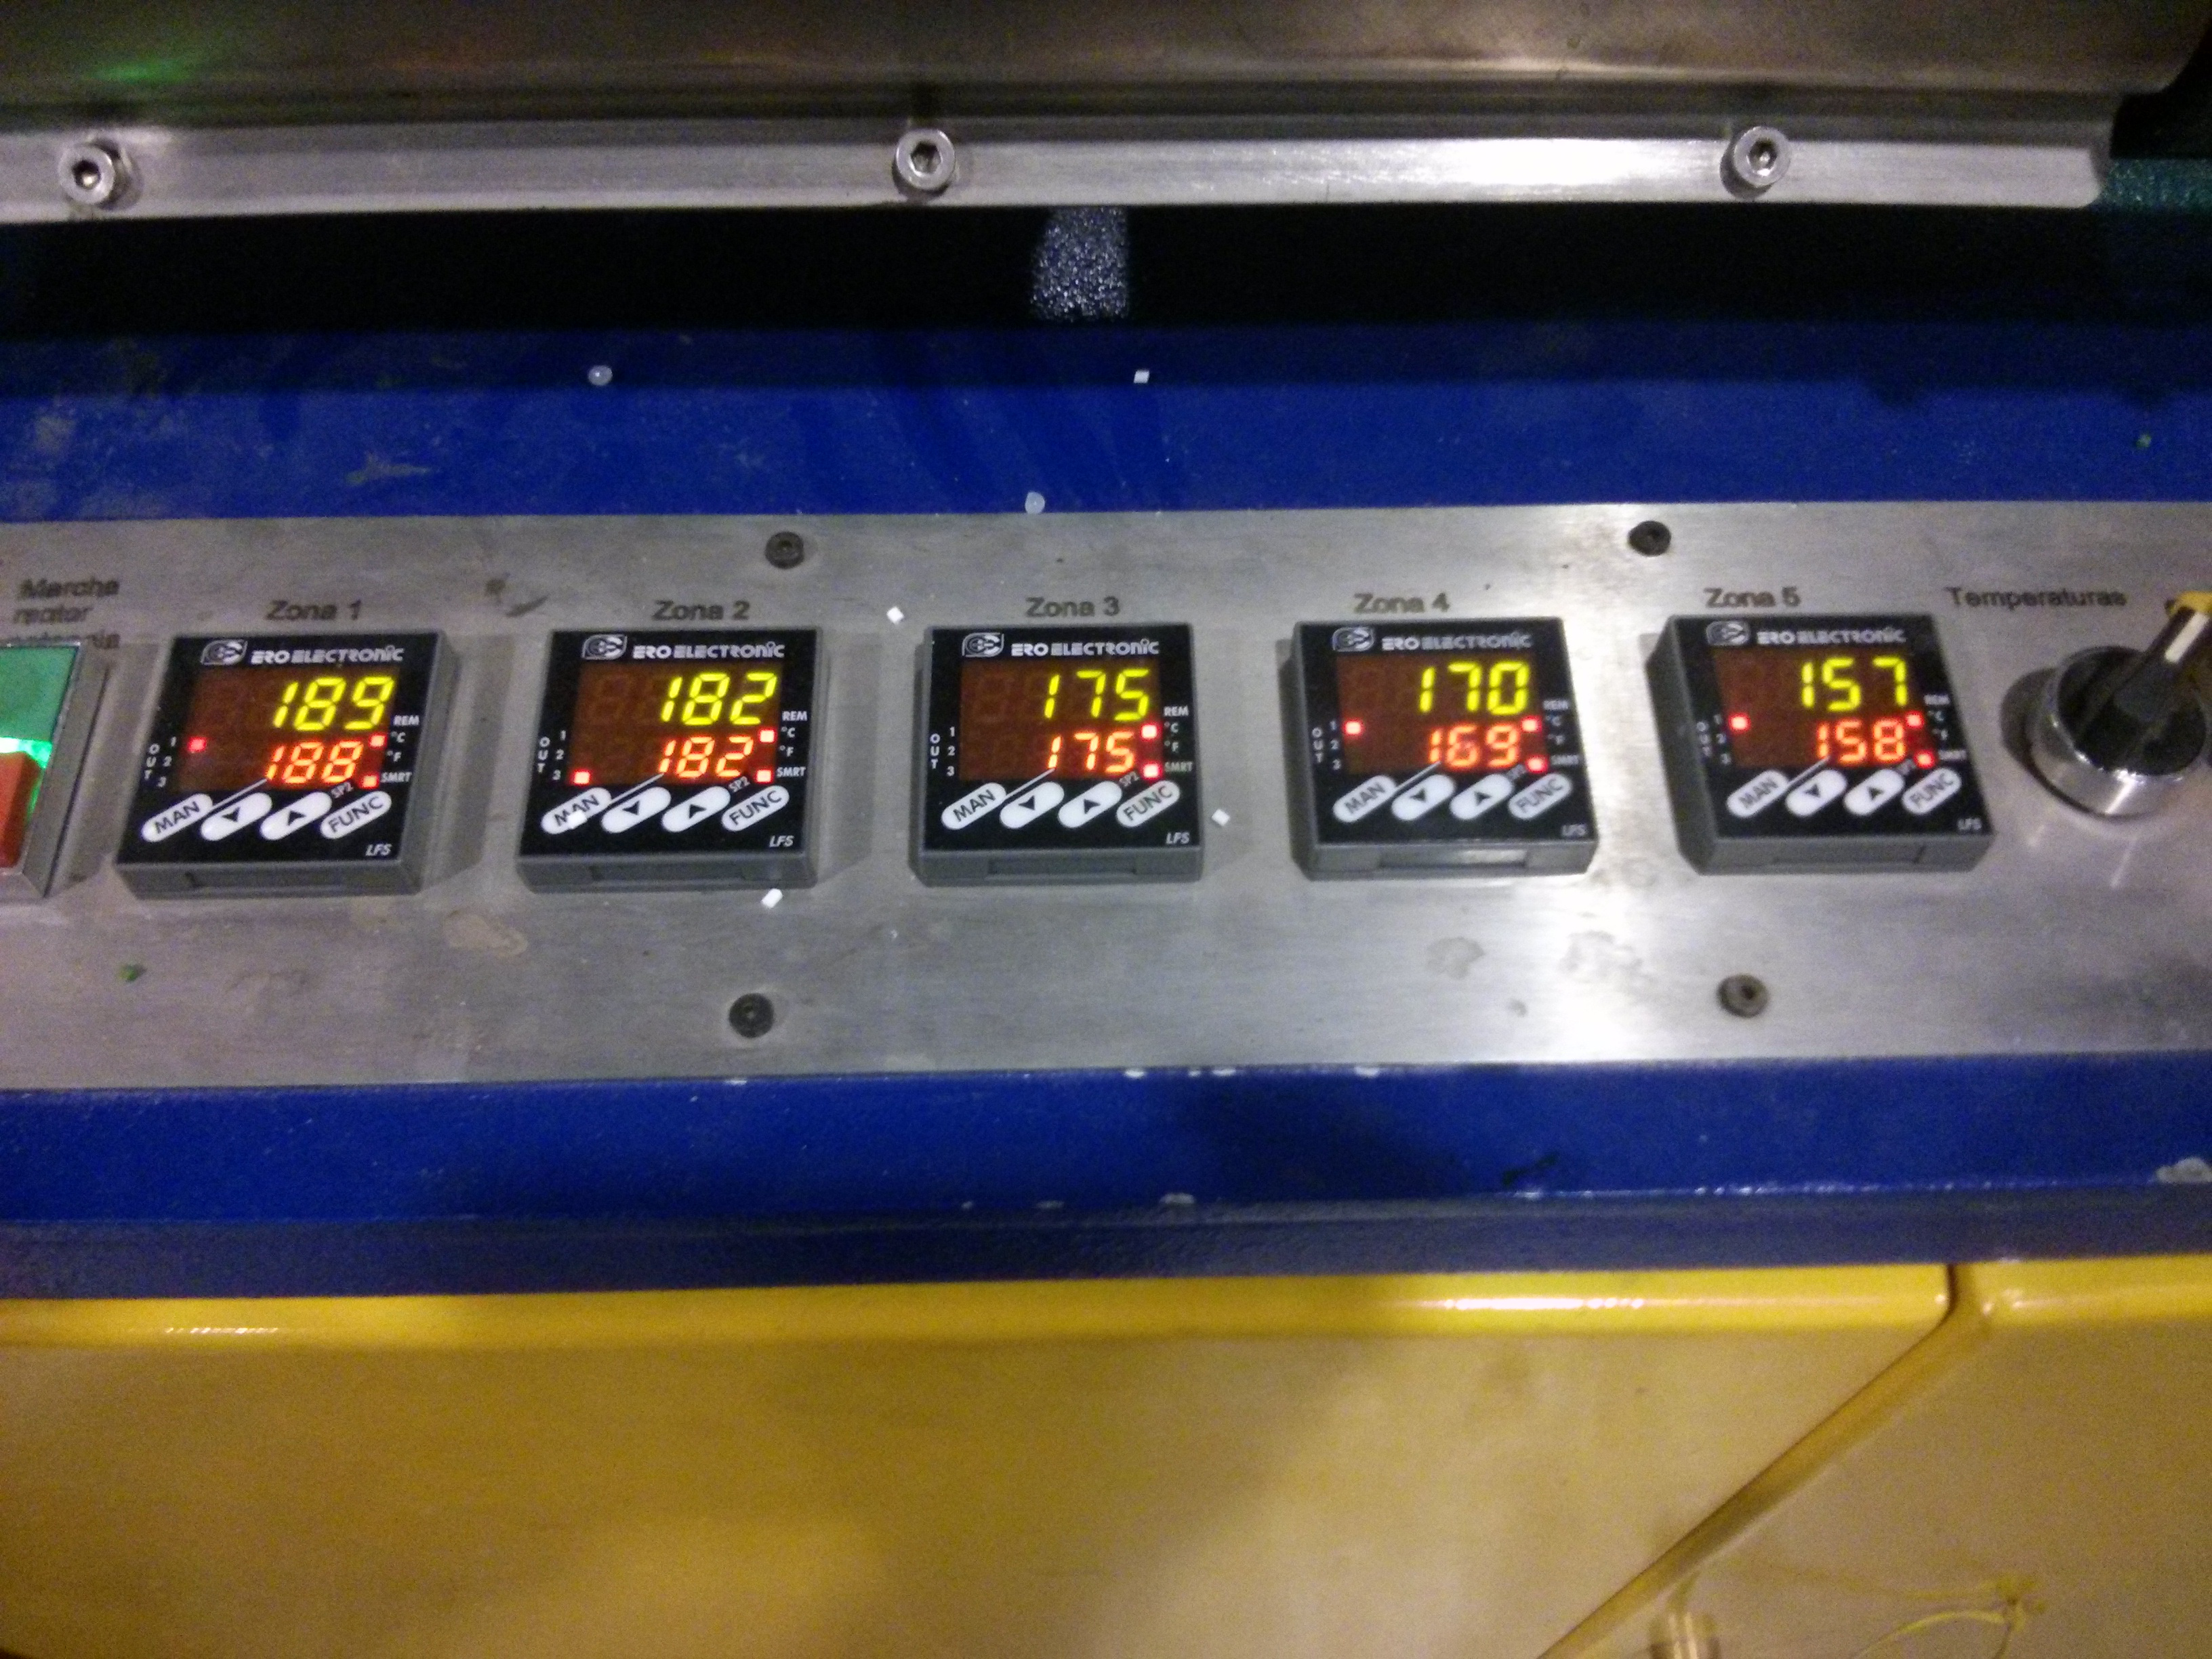
\includegraphics[width=0.4\textwidth]{images/huesca/IMG_20141216_175204.jpg}
            \caption{Sensores de temperatura}
            \label{fig:hardware_temperatura}
    \end{figure}

Buscando en internet referencias de los posibles componentes que disponemos, y con ayuda de los responsables de la fábrica, llegamos a la conclusión de que el hardware que disponemos es el siguiente:

\begin{itemize}
	\item \textbf{Reguladores temperatura Extrusora:} 5x Eroelectronic LFS
	\item \textbf{Regulador temperatura bañera:} 1x OMRON E5CC
	\item \textbf{Bobinadora: IO distribuidas: }
	\begin{itemize}

       \item {SmartStix I/O:} HE559DQM706B y HE559DI710B
       \item{HMI:} HE-XT351C112CF
        \item{Variador (control tractora):} Optidrive rrp2 ODP-24400-SP
        \item{Sensor diámetro:} conectado a módulo Adam 6066
        	\begin{itemize}
        				\item Omron ZX-GIF41 (RS232)
        				\item Omron ZX-GTC41 (Controlador)
                        \item Omron ZX-GT28S41 (sensor)
             \end{itemize}
        \item Relés: OMRON MY2IN
    \end{itemize}
\end{itemize}

Así mismo, disponemos de los datasheet y sabemos qué tipo de comunicación podemos disponer con cada uno, información necesaria para poder establecer la arquitectura del sistema.

\section{Arquitectura planteada}
\label{arquitectura}

Antes de plantear la arquitectura, deberemos establecer el protocolo de comunicaciones y el medio físio por el que irán conectados entre sí. Mirando las especificaciones de los componentes llegamos a la siguiente conclusión

\begin{table}[]

\begin{tabular}{ccc}
\hline
{\bf Dispositivo}     & {\bf Protocolo} & {\bf Medio} \\ \hline
Senores temperatura   & Modbus          & RS485       \\
Pantalla HMI          & Modbus          & RS485       \\
Adam                  & Modbus-TCP      & RS485       \\
Sensor diámetro       & -               & RS232       \\
Variador              & Modbus-TCP      & RS485       \\
Perifería distribuida & CsCAN           & Modbus      \\
Bobinadora            &                 & Cableado    \\ \hline
\end{tabular}
\centering
\caption{My caption}
\label{my-label}
\end{table}


 	\begin{figure}[H]
            \centering
            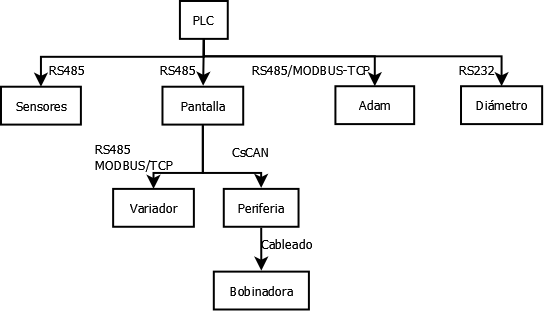
\includegraphics[width=0.6\textwidth]{images/20141229.png}
            \caption{Arquitectura propuesta}
            \label{fig:hardware_arquitectura}
    \end{figure}

\section{Programación del PLC}
\label{sec:program.plc}

Para la programación del PLC se usará el software de desarrollo que proporciona la compañía ABB en su web\footnote{http://new.abb.com/plc/automationbuilder/platform/software}. La versión usada en este proyecto del Automation Builder es la última liberada hasta la fecha, la 1.1.0.824, como se indicó en la sección \ref{eleccion_PLC} este software es gratuito para el uso que le vamos a dar.\\
    \begin{figure}[H]
            \centering
            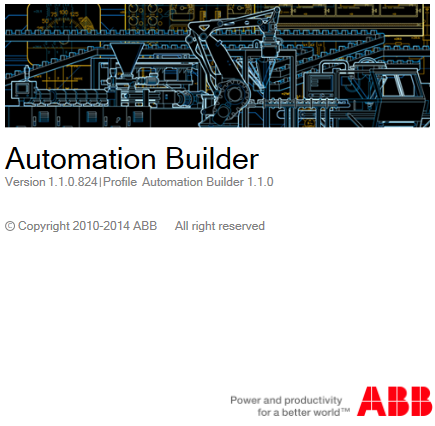
\includegraphics[width=0.4\textwidth]{images/PLC/ABB.png}
            \caption{Splash Screen del Automation Builder}
            \label{fig:PLC_splashabb}
    \end{figure}
Las acciones que debe realizar el PLC son las siguientes:

\begin{itemize}
	\item{Controlar la temperatura del extrusor.}
	\item{Controlar motor del husillo.}
	\item{Leer información del sensor de diámetro.}
	\item{Almacenar la información tomada en un fichero de datos.}
	\item{Visualizar en una página web el estado de la producción.}
\end{itemize}

Para realizar el software que gestione el PLC, se usará una máquina de estados, en la que pasando por diversas fases, se irán ejecutando las acciones de control. Deberemos entrar en modo producción mediante la activación de una variable, con la que si estamos en producción, pasaremos por los distintos estados, mientras no estemos en producción, las salidas digitales y valores de consigna de los PID, estarán reseteados a cero como medida de seguridad. Una vez que entremos en producción, el primer paso será inicializar el programa, generaremos el nombre del fichero donde almacenaremos los datos. Se elije un nombre en el que se usa año, mes, día y minuto para identificar la producción, es decir, tendría un formato \textit{YYMMDDmm.CSV}.\\

El formato elegido para almacenar la información es el de valores separados por coma (CSV). El motivo por el cual se elije este formato es debido a su estandarización y que almacena los datos de forma tabular en texto plano. Gracias a esto, podremos abrir el fichero CSV con cualquier editor de texto y otros programas de hojas de cálculo, para el posterior análisis de los datos, que es uno de los objetivos del proyecto. Por lo tanto, el formato CSV es el idóneo para poder trabajar en el futuro con los datos almacenados.\\

En esta inicialización, también se genera la cabecera del fichero CSV , que es la primera fila del fichero, en donde indicará la información que contiene cada columna. La información almacenada en el fichero CSV será la siguiente:

\begin{itemize}
	\item{\textbf{Time Stamp: }Es una secuencia de caracteres en las que se indican hora y fecha de un evento ocurrido. Se almacena con el  formato YY-MM-DD HH:MM:SS. Con esta información podremos tener una trazabilidad del filamento almacenado y en caso de producirse un error, ver el momento concreto del mismo.}
	\item{\textbf{Temperaturas: }Valores con las temperaturas del dado y el husillo en la zona de alimentación. De esta manera se comprueba que la temperatura no sufre algún cambio drástico durante el proceso, que puede ser causante de un problema en la calidad final del filamento (X e Y).}
	\item{\textbf{Diámetros: }Se almacenan los diámetros medidos por el sensor. En este caso se van a poner dos sensores de diámetro para hacer una medición en los dos ejes del filamento.}
	\item{\textbf{Información varia: }Se puede almacenar cualquier información que nosotros deseemos en un futuro.}
\end{itemize}

Los siguientes pasos dentro de la máquina de estados, será generar el fichero CSV y en caso de que no se produzca ningún error,	 se almacenará la cabecera en el fichero CSV, para pasar a la producción como tal.\\
Se controlará la temperatura del dado, se registrarán los valores de diámetros y temperaturas y se irán almacenando en el fichero CSV. El control del motor del husillo se hará de forma manual desde la visualización online.\\

Una vez que se tiene una idea de cómo va a ser el programa, se desarrolla un diagrama con la máquina de estados.

    \begin{figure}[H]
            \centering
            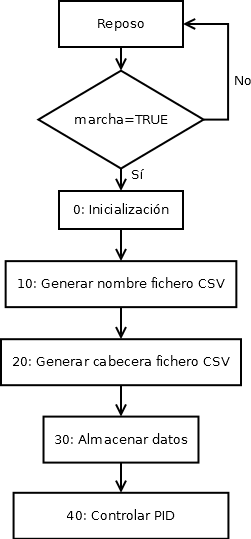
\includegraphics[width=0.25\textwidth]{images/PLC/diagrama.png}
            \caption{Diagrama de estados}
            \label{fig:plc_estados}
    \end{figure}


\subsection{Controlar temperatura extrusor}
\label{sec:plc_PID}

Para controlar la temperatura del extrusor se va a implementar un regulador PID. Los reguladores del tipo PID, añaden tres acciones de regulación,... BLA BLA BLA BLA BLA BLA\cite{PID}\\


Para poder implementar correctamente un regulador PID, será necesario conocer la planta del sistema que queremos regular. En nuestro caso es el sistema de calentamiento del dado, por ello, deberemos modelar primeramente el sistema con el que estamos trabajando.
    \begin{figure}[H]
            \centering
            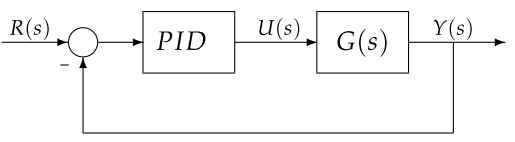
\includegraphics[width=0.4\textwidth]{images/PLC/sistema.png}
            \caption{Sistema con un regulador PID}
            \label{fig:plc_sistema}
    \end{figure}

Con ayuda del programa que estamos desarrollando en el PLC haremos las siguientes tareas:

\begin{itemize}
	\item{Registrar temperaturas del dado.}
	\item{Encender de forma controlada la resistencia de calentamiento.}
	\item{Analizar los datos obtenidos.}
\end{itemize}

Tenemos que ver como se comporta el sistema en lazo abierto, sin ningún tipo de control. Partiendo de una temperatura ambiente, se irán registrando los valores de las temperaturas para a continuación encender la resistencia de calentamiento y ver cómo la temperatura va aumentando a medida que pasa el tiempo. Una vez que la temperatura sobrepase un valor que nosotros establezcamos, pararemos el experimento.\\

Con ayuda del lenguaje de programación Python y varias herramientas de análisis de datos como son: ipython,scipy, pandas y numpy, analizaremos los datos obtenidos. Las gráficas peresentadas a continuación, así como los cálculos están realizadas con esta herramienta.

    \begin{figure}[H]
            \centering
            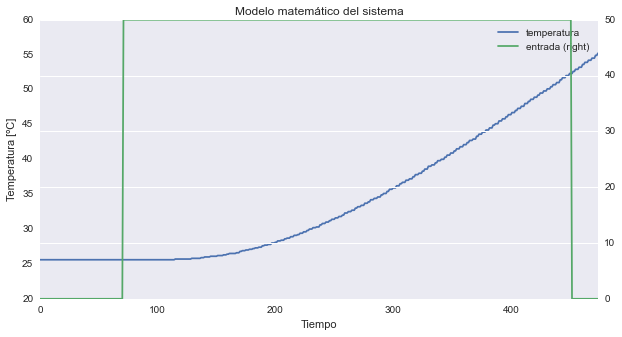
\includegraphics[width=0.75\textwidth]{images/PLC/modelado/modelado_9_1.png}
            \caption{Respuesta del sistema en lazo abierto}
            \label{fig:plc_lazo_abierto}
    \end{figure}

Calcularemos cual es la ecuación que mejore se ajuste a nuestros datos y tendremos el polinomio que caracteriza nuestro sistema.
    \begin{figure}[H]
            \centering
            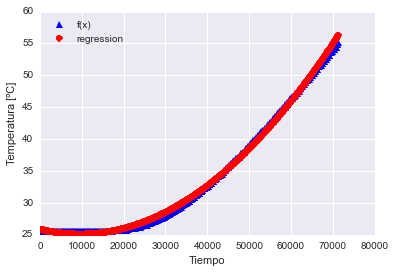
\includegraphics[width=0.5\textwidth]{images/PLC/modelado/modelado_13_1.png}
            \caption{Ajuste de la recta}
            \label{fig:plc_lazo_abierto2}
    \end{figure}
$$P_x=  25.9459 -1.5733 \cdot 10^{-4} \cdot X - 8.18174 \cdot 10^{-9} \cdot X^2$$

Si calculamos la transformada de laplace del sistema, obtenemos la planta de nuestro sistema, con la cual podremos implementar el regulador PID:
$$G_s = \frac{25.95 \cdot S^2 - 0.00015733 \cdot S + 1.63635 \cdot 10^{-8}}{S^3}$$

Aplicando el método de sintonizacion de Ziegler-Nichols basado en la curva reacción calcularemos el PID para poder regular correctamente el sistema.Este método consiste en estudiar el sistema en lazo abierto con escalón unitario, calculamos parámetros como la máxima pendiente de la curva y el retardo, y establecemos con ellos las ganancias del controlador PID\cite{PID}.Nos da de manera rápida unos valores de $K_p$, $K_i$ y $K_d$ orientativos, para que podamos ajustar correctamente el controlador. Con ayuda de la herramienta Open Source Octave, calcularemos los valores de ganancia que serán los que apliquemos a nuestro regulador.

\Cpp
\begin{lstlisting}
pkg load control
%los datos en la funcion tf() debe ser el numerador y denominador de nuestro sistema.
H=tf([25.95 0.000157333 1.63635E-8],[1 0 0 0]);
step(H);
dt=0.150;
t=0:dt:65;
y=step(H,t);
dy=diff(y)/dt;
[m,p]=max(dy);
yi=y(p);
ti=t(p);
L=ti-yi/m
Tao=(y(end)-yi)/m+ti-L
Kp=1.2*Tao/L
Ti=2*L;
Td=0.5*L;
Ki=Kp/ti;
Kd=Kp*Td;
\end{lstlisting}

En esta primera iteración, los datos obtenidos son los siguientes:
$K_p = 6082.6$ $K_i=93.868 K_d=38.9262$

Con lo que nuestro regulador tiene la siguiente ecuación característica:

$$G_s = \frac{38.9262 \cdot S^2 + 6082.6 \cdot S + 93.868}{S}$$

Una vez que tenemos las ganancias de nuestro regulador PID, volvemos a realizar el experimento de calentar la resistencia hasta un valor de temperatura deseado, en este caso 80ºC y vemos cual es la respuesta de nuestro sistema:

    \begin{figure}[H]
            \centering
            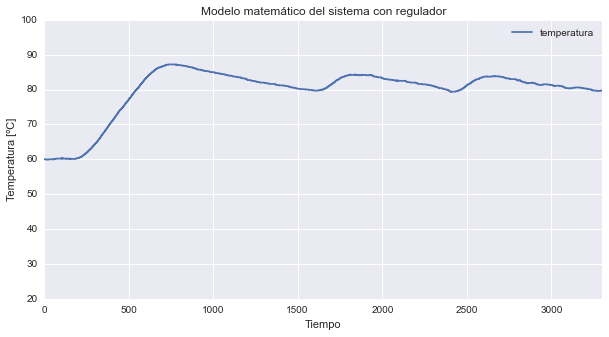
\includegraphics[width=0.75\textwidth]{images/PLC/modelado/modelado_26_1.png}
            \caption{Respuesta del sistema con PID. Iteracción 1}
            \label{fig:plc_PID1}
    \end{figure}

Como podemos objservar en la imagen \ref{fig:plc_PID1} tenemos una sobreoscilación sobre el setpoint elevada:

$$M_{p}=\frac{T_{max}-Setpoint}{Setpoint} \cdot 100 = \frac{87.20-80}{80} \cdot 100 = 9\%$$ 

Siendo el error en régimen  permanente de 3.70.\\
Una vez introducido el controlador, la temperatura tiende a estabilizarse, sin embargo tiene mucha sobreoscilación. Por ello aumentaremos los valores de $K_i$ y $K_d$, siendo los valores de esta segunda iteracción los siguientes:
$K_p = 6082.6$ $K_i=103.25 K_d=51.425$


Realizando una segunda iteracción en el cálculo de nuestro regulador obtenemos lo siguiente:

    \begin{figure}[H]
            \centering
            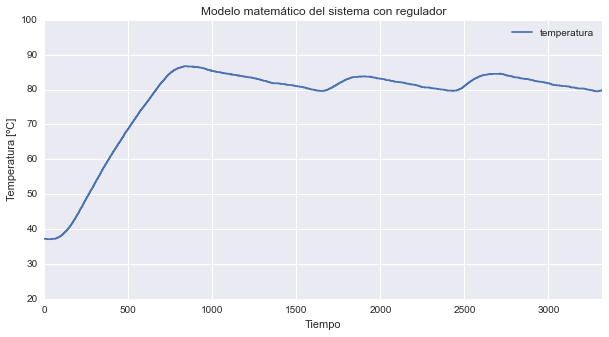
\includegraphics[width=0.75\textwidth]{images/PLC/modelado/modelado_30_1.png}
            \caption{Respuesta del sistema con PID. Iteracción 2}
            \label{fig:plc_PID2}
    \end{figure}
Esta vez los resultados son algo mejores:
$$M_{p}=\frac{T_{max}-Setpoint}{Setpoint} \cdot 100 = \frac{86.70-80}{80} \cdot 100 = 8.38\%$$ 
Siendo el error en régimen permanente de 3.50.\\
En esta segunda iteracción hemos logrado bajar la sobreoscilación inicial, pero tenemos mayor error en regimen permanente. Por ello volvemos a aumentar los valores de $K_i$ y $K_d$ siendo los valores de esta tercera iteracción los siguientes:
$K_p = 6082.6$ $K_i=121.64 K_d=60$

Realizando una tercera iteracción en el cálculo de nuestro regulador obtenemos lo siguiente:

    \begin{figure}[H]
            \centering
            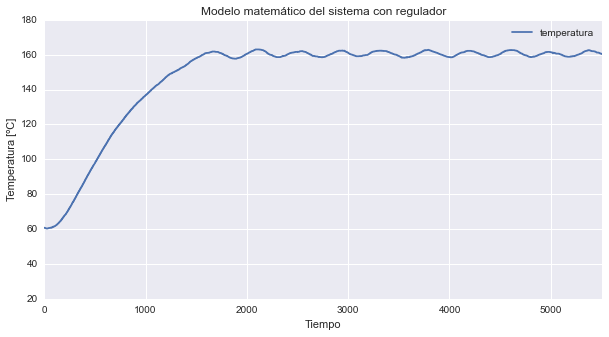
\includegraphics[width=0.75\textwidth]{images/PLC/modelado/modelado_34_1.png}
            \caption{Respuesta del sistema con PID. Iteracción 3}
            \label{fig:plc_PID3}
    \end{figure}
Esta vez los resultados son algo mejores:
$$M_{p}=\frac{T_{max}-Setpoint}{Setpoint} \cdot 100 = \frac{163-160}{160} \cdot 100 = 1.88\%$$ 
Siendo el error en régimen permanente de 1.30\\
En este caso, se puso un setpoint de 160ºC. Como vemos, la sobreoscilación inicial ha disminuido en comparación con la anterior iteracción y el error en regimen permanente es menor. Para intentar minimar el error, aumentaremos únicamente el valor de $K_i$. Siendo los valores de esta cuarta iteracción del regulador los siguientes:
    $K_p = 6082.6$ $K_i=121.64 K_d=150$

Realizando una cuarta iteracción en el cálculo de nuestro regulador obtenemos lo siguiente:

    \begin{figure}[H]
            \centering
            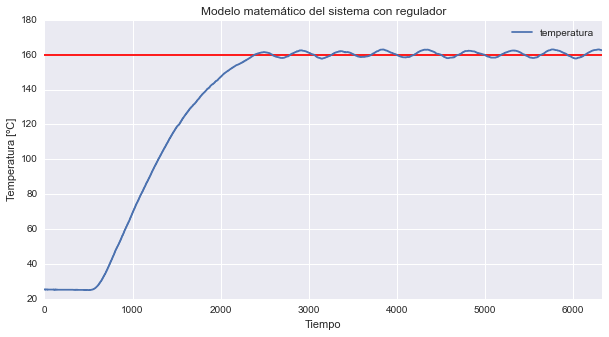
\includegraphics[width=0.75\textwidth]{images/PLC/modelado/modelado_38_1.png}
            \caption{Respuesta del sistema con PID. Iteracción 4}
            \label{fig:plc_PID4}
    \end{figure}
Esta vez los resultados son algo mejores:
$$M_{p}=\frac{T_{max}-Setpoint}{Setpoint} \cdot 100 = \frac{163-160}{160} \cdot 100 = 1.88\%$$ 
Siendo el error en régimen permanente de 1.10\\

Por lo tanto, el regulador que cumple con las especificaciones deseadas tiene la siguiente ecuación característica:
$$G_s = \frac{150 \cdot S^2 + 6082.6 \cdot S + 121.64}{S}$$

\subsection{Leer información del sensor de diámetro}
\label{sec:plc_diametro}

Los sensores de diámetro están conectados a dos entradas analógicas de tensión del PLC. Será necesario unir la señal de masa (GND) del PLC con la del sensor, para que la referencia al nivel de tensión 0v sea la misma, posteriormente, la salida del sensor de diámetro, se conectará con la entrada analógica del PLC.\\

El PLC convierte el valor de tensión comprendido entre un rango de 0-10V a un valor numérico, a través de un conversor analógico a digital (ADC) de 10bits, es decir, tenemos una resolución de:

$$ Resolucion=\frac{ V_{max} } {2^{10} } = \frac{10}{1024} = 9.76 mV$$

Si acudimos a la ayuda que nos ofrece el programa de ABB, podemos observar los valores que asigna el ADC:

\begin{table}[H]
\centering
\begin{tabular}{|c|c|c|}
\hline
{\bf Intervalo}                   & {\bf 0 ... 10V}                                                   & \multicolumn{1}{l|}{{\bf Valor digital}}                       \\ \hline
Desbordamiento                    & \textgreater 11.7589                                              & 32767                                                         \\ \hline
Valor de medición desmasiado alto & \begin{tabular}[c]{@{}c@{}}11.7589\\ .\\ .\\ 10.0004\end{tabular} & \begin{tabular}[c]{@{}c@{}}32511\\ .\\ .\\ 27649\end{tabular} \\ \hline
Intervalo normal                  & \begin{tabular}[c]{@{}c@{}}10.000\\ .\\ .\\ 0.0004\end{tabular}   & \begin{tabular}[c]{@{}c@{}}27648\\ .\\ .\\ 1\end{tabular}     \\ \hline
\end{tabular}
\caption{Valores de conversión del ADC}
\label{tab:reso_adc}
\end{table}

En nuestro caso, vamos a trabajar en el rango de intervalo normal, para poder saber el diámetro que nos está dando el sensor, deberemos leer la entrada analógica y convertir el valor décimal a un valor de tensión, es decir, convertir el valor digital a analogico, (DAC), para ello, cogemos los valores del intervalo normal de la tabla \ref{tab:reso_adc} y calcular la ecuación de la recta que lo caracteriza.

    \begin{figure}[H]
            \centering
            \includegraphics[width=0.75\textwidth]{images/PLC/dac.png}
            \caption{Ecuación: $Y=3.6168 \cdot 10^{-4} \cdot X$}
            \label{fig:plc_DAC}
    \end{figure}

Con este valor, y el calculado en \pageref{fig:sens_regre} somos capaces de leer el valor del diámetro, para ello, prograremos un bloque que llamaremos linealizacion, en la que tendrá los siguientes parámetros:

\begin{itemize}
    \item{\textbf{Entradas:}}
        \begin{itemize}
            \item{\textbf{IN:}Entrada analógica donde se encuentra físicamente el sensor}
            \item{\textbf{AD:}Valor del DAC calculado anteriormente}
            \item{\textbf{M y B:} Valores de la ecuación de la recta, que minimizan el error medido por el sensor}         
        \end{itemize}
    \item{\textbf{Salida:}}
        \begin{itemize}
            \item{\textbf{OUT:} Valor real de la magnitud medida por el sensor.}
        \end{itemize}
\end{itemize}
%\chapter{Montaje filawinder}
\label{ane:filawinder}
Para poder almacenar el filamento que vamos extruyendo mediante el Filastruder hemos escogido un kit DIY, llamado Filawinder\cite{filawinder}. 

    \begin{figure}[H]
            \centering
            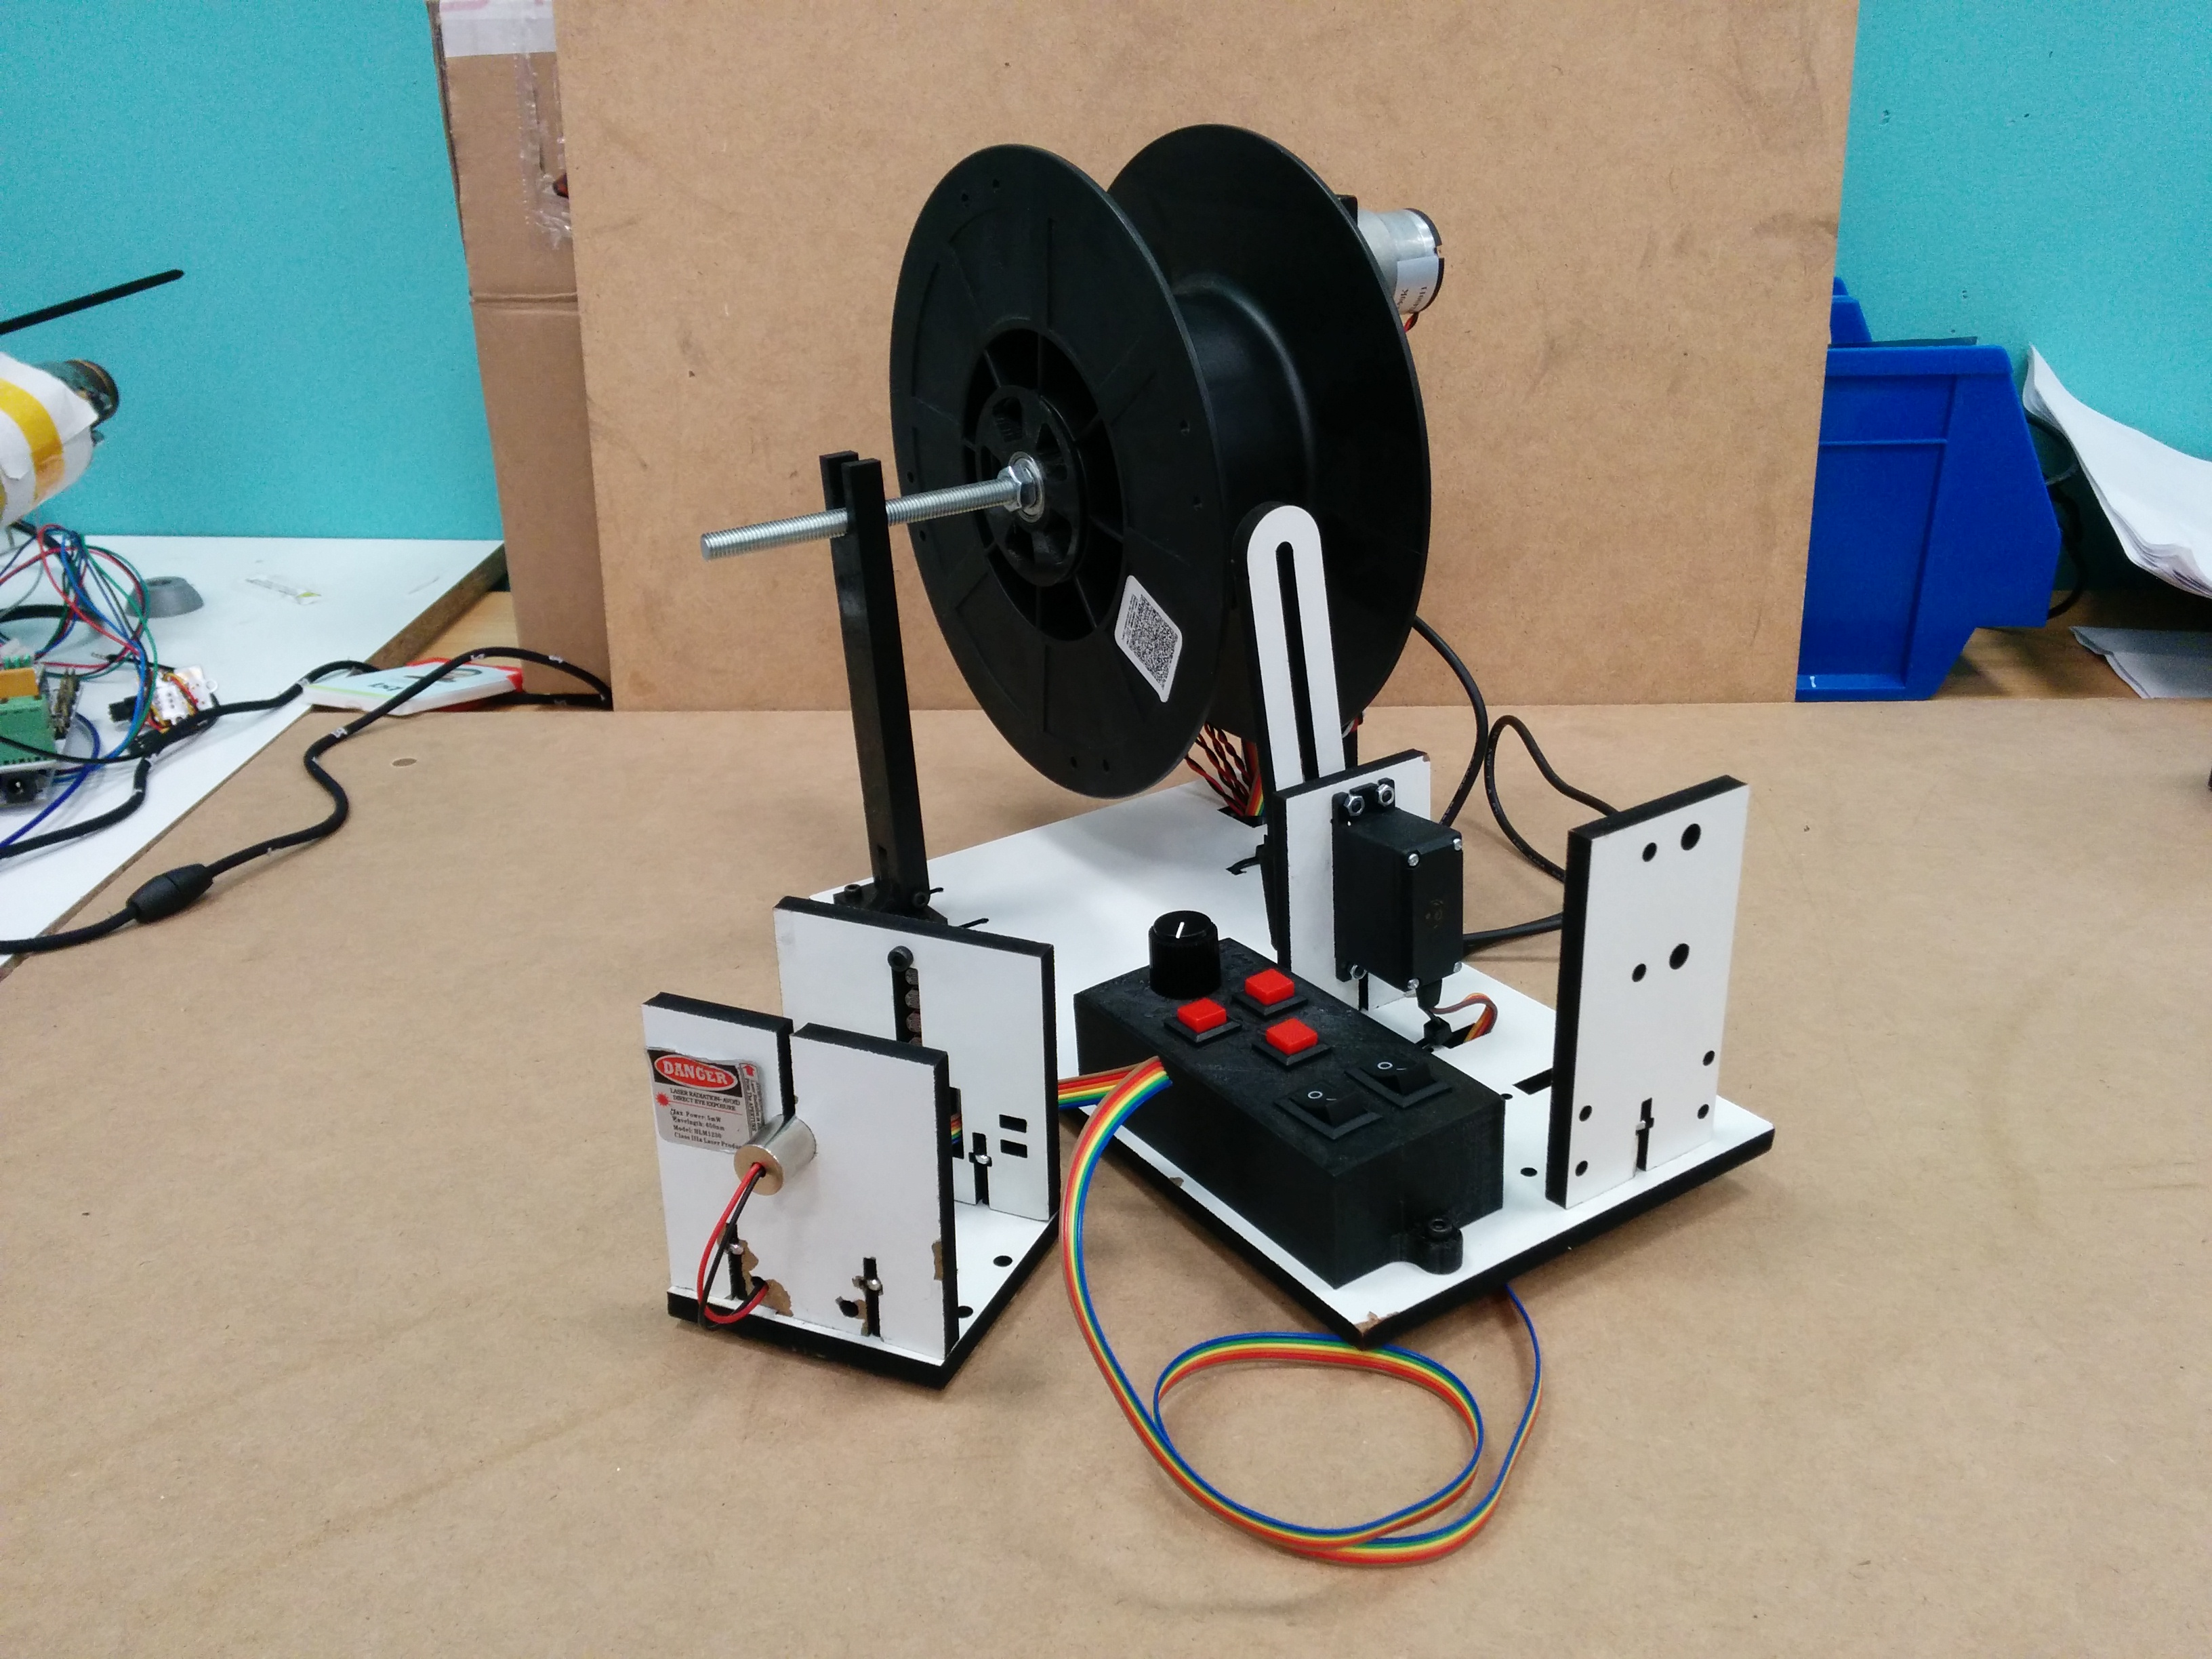
\includegraphics[width=0.4\textwidth]{images/filawinder/IMG_20150313_103643.jpg}
            \caption{Montaje de Filawinder.}
            \label{fig:winder_winder}
    \end{figure}

Filawinder es un kit DIY que se ofrece como expansión a la extrusora  filaextruder. Hemos elegido este en concreto debido a su similitud con una bobinadora de filamento real haciendo así, que la maqueta que vamos a montar sea lo más cercana a la realidad. Otra ventaja es su facilidad de montaje y la amplia documentación disponible en Internet.\\

Filawinder es un sistema de almacenamiento de bobinado automatizado. Consiste en un motor en el que va anclado la bobina para almacenar el filamento. La velocidad de giro del motor, está controlada por unos sensores de posición que detectan la tensión del filamento, y en función de ello la velocidad del motor es regulada. Estos sensores resistivos de luz (LDR), funcionan mediante la proyección de la sombra del filamento en ellos para que su resistencia varíe. El filamento, al pasar entre medias del haz y los LDR, irá proyectando la sombra y podremos detectar la tensión del filamento. Logrando así mejorar el almacenamiento del filamento producido.

    \begin{figure}[H]
            \centering
            \includegraphics[width=0.4\textwidth]{images/filawinder/Sensor-filamento.jpg}
            \caption{Sensor de filamento.}
            \label{fig:winder_sensor}
    \end{figure}

También dispone de una guía automática que va moviendo el filamento a lo largo de la bobina, para evitar nudos en su bobinado. Esta guía va teniendo en cuenta el número de vueltas que va realizando la bobina, para ir desplazando el filamento a lo largo del eje transversal de la bobina.\\

Filawinder se distribuye en formato DIY por lo que se venden las piezas sueltas y es necesario que el usuario final realice el montaje. (Ver imagen \ref{fig:winder_material})
    \begin{figure}[H]
            \centering
            \includegraphics[width=0.5\textwidth]{images/filawinder/materiales-filawinder.png}
            \caption{Materiales de filawinder.}
            \label{fig:winder_material}
    \end{figure}

Además de las piezas que se nos suministra, también será necesario tener acceso a una impresora 3D para imprimir unas piezas necesarias para completar el montaje.

    \begin{figure}[H]
            \centering
            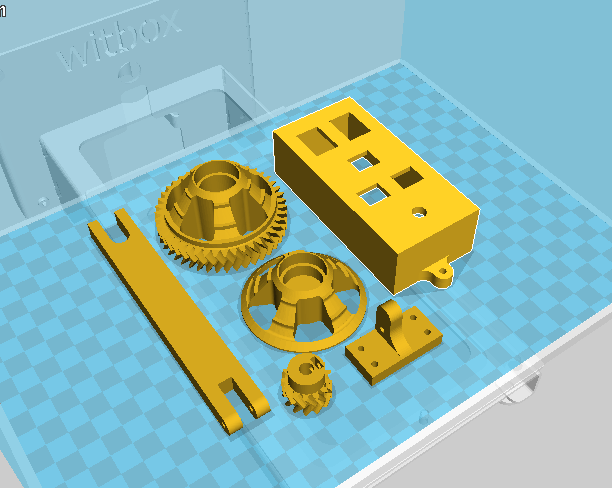
\includegraphics[width=0.5\textwidth]{images/filawinder/piezas-impresas.png}
            \caption{Piezas impresas para filawinder.}
            \label{fig:winder_piezas}
    \end{figure}

 Una vez que ya tenemos todas las piezas disponibles, podremos empezar con el montaje.\\

Alojamos el motor en la pieza destinada a ello. Con ayuda de dos tornillos M3X10 sujetamos el motor a la pieza para evitar que se mueva, pero no hacemos mucha fuerza, ya que la posición final se realizará más adelante.

    \begin{figure}[H]
            \centering
            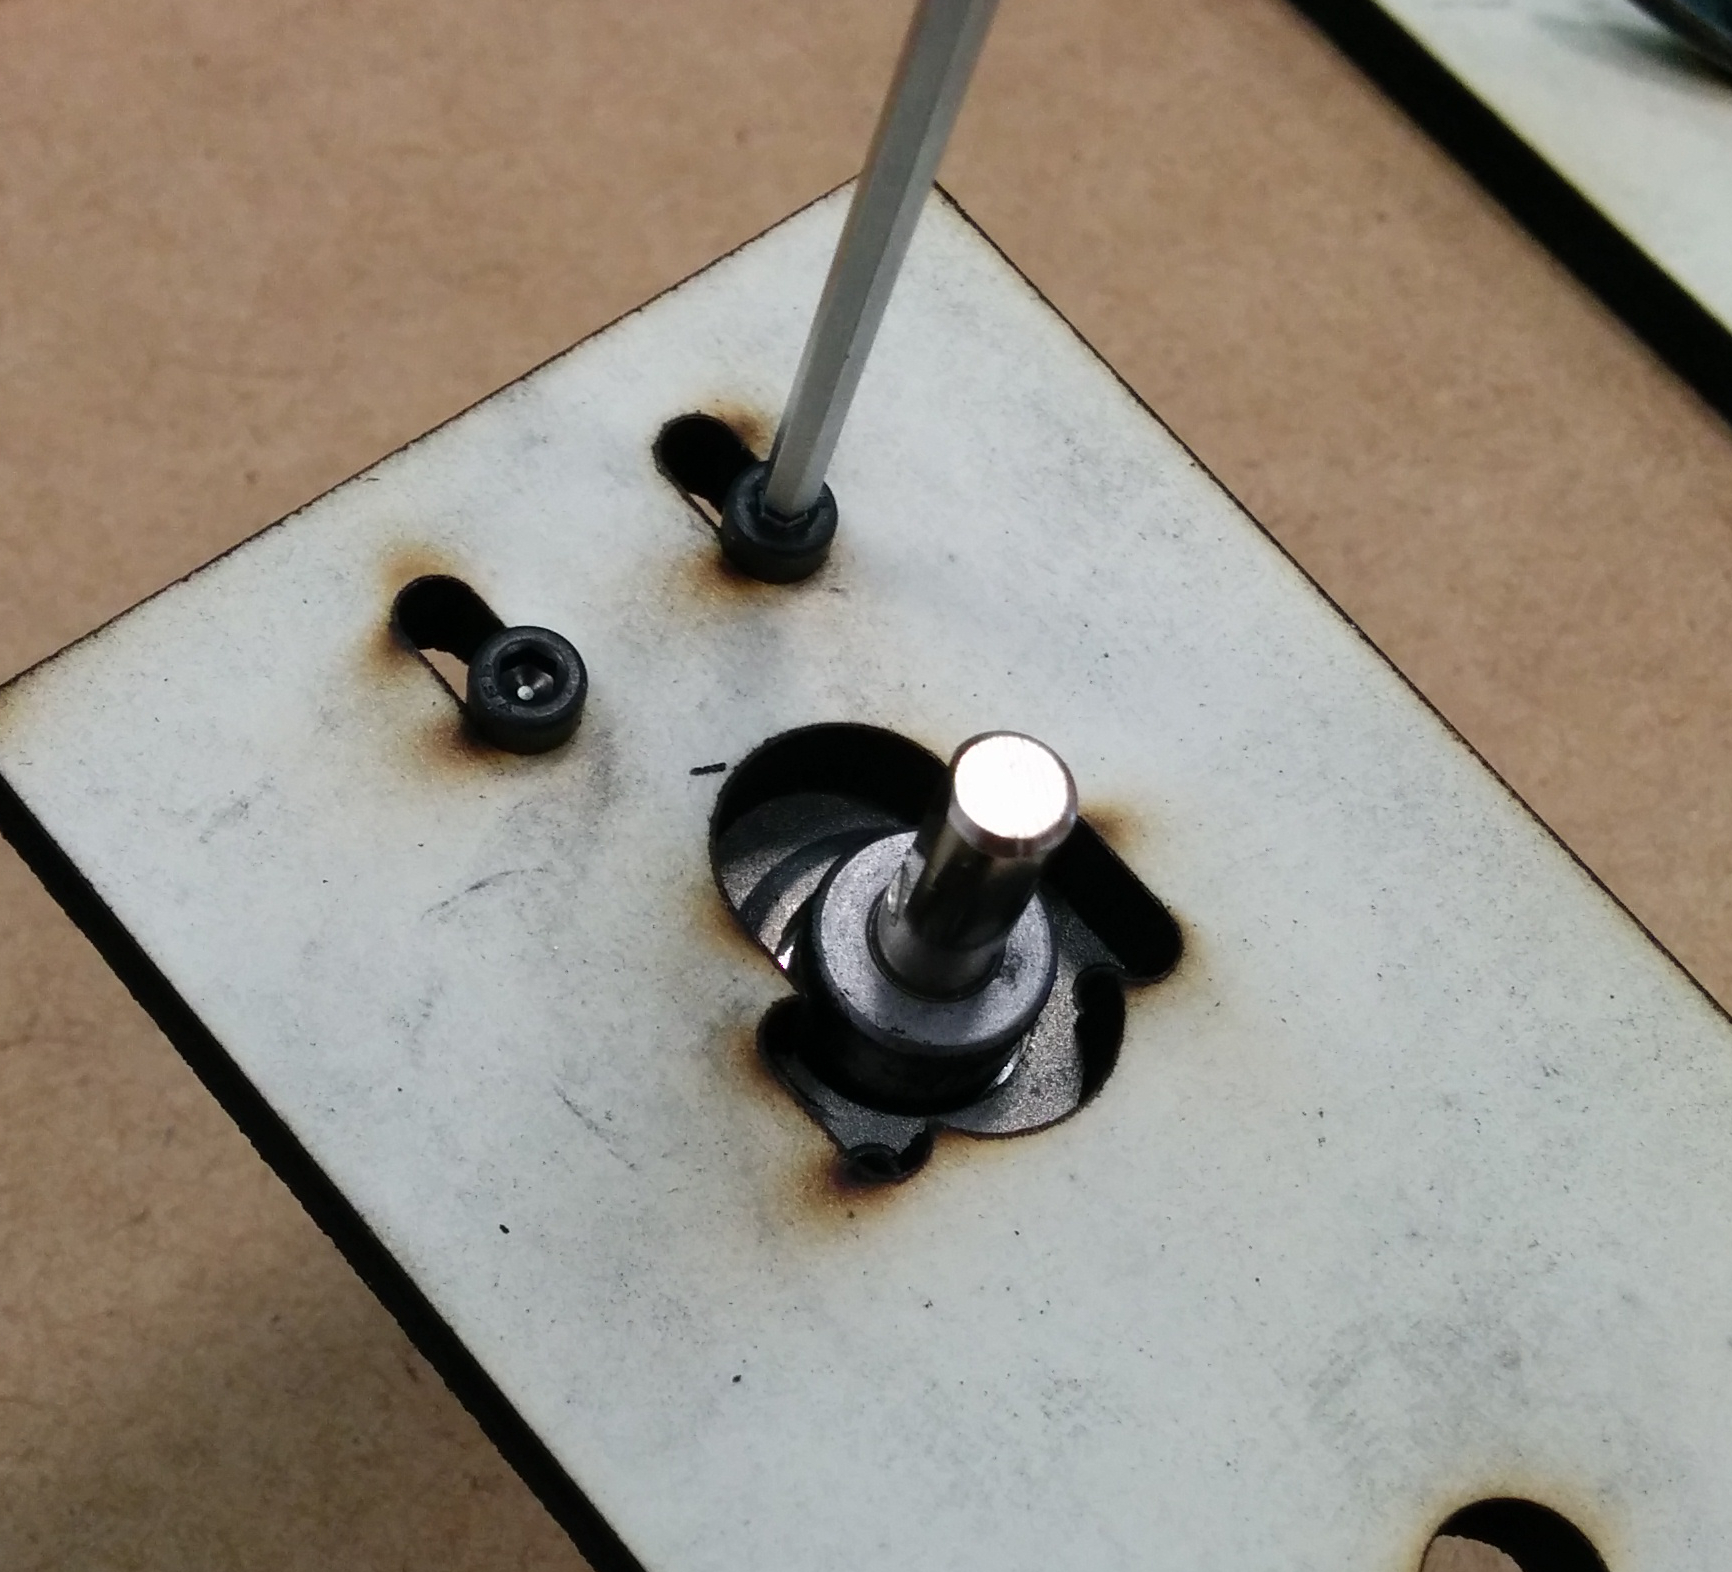
\includegraphics[width=0.5\textwidth]{images/filawinder/montaje1.png}
            \caption{Introducimos el motor en el hueco.}
            \label{fig:winder_piezas1}
    \end{figure}

    Introducimos una tuerca en el alojamiento del engranaje pequeño como se ve en la imagen \ref{fig:winder_engranaje}, para poder apretar el engranaje al vástago del motor con el tornillo de M3x10 (Ver imagen \ref{fig:winder_apriet})
    \begin{figure}[H]
          \centering
        \begin{subfigure}[b]{0.35\textwidth}
                \centering
                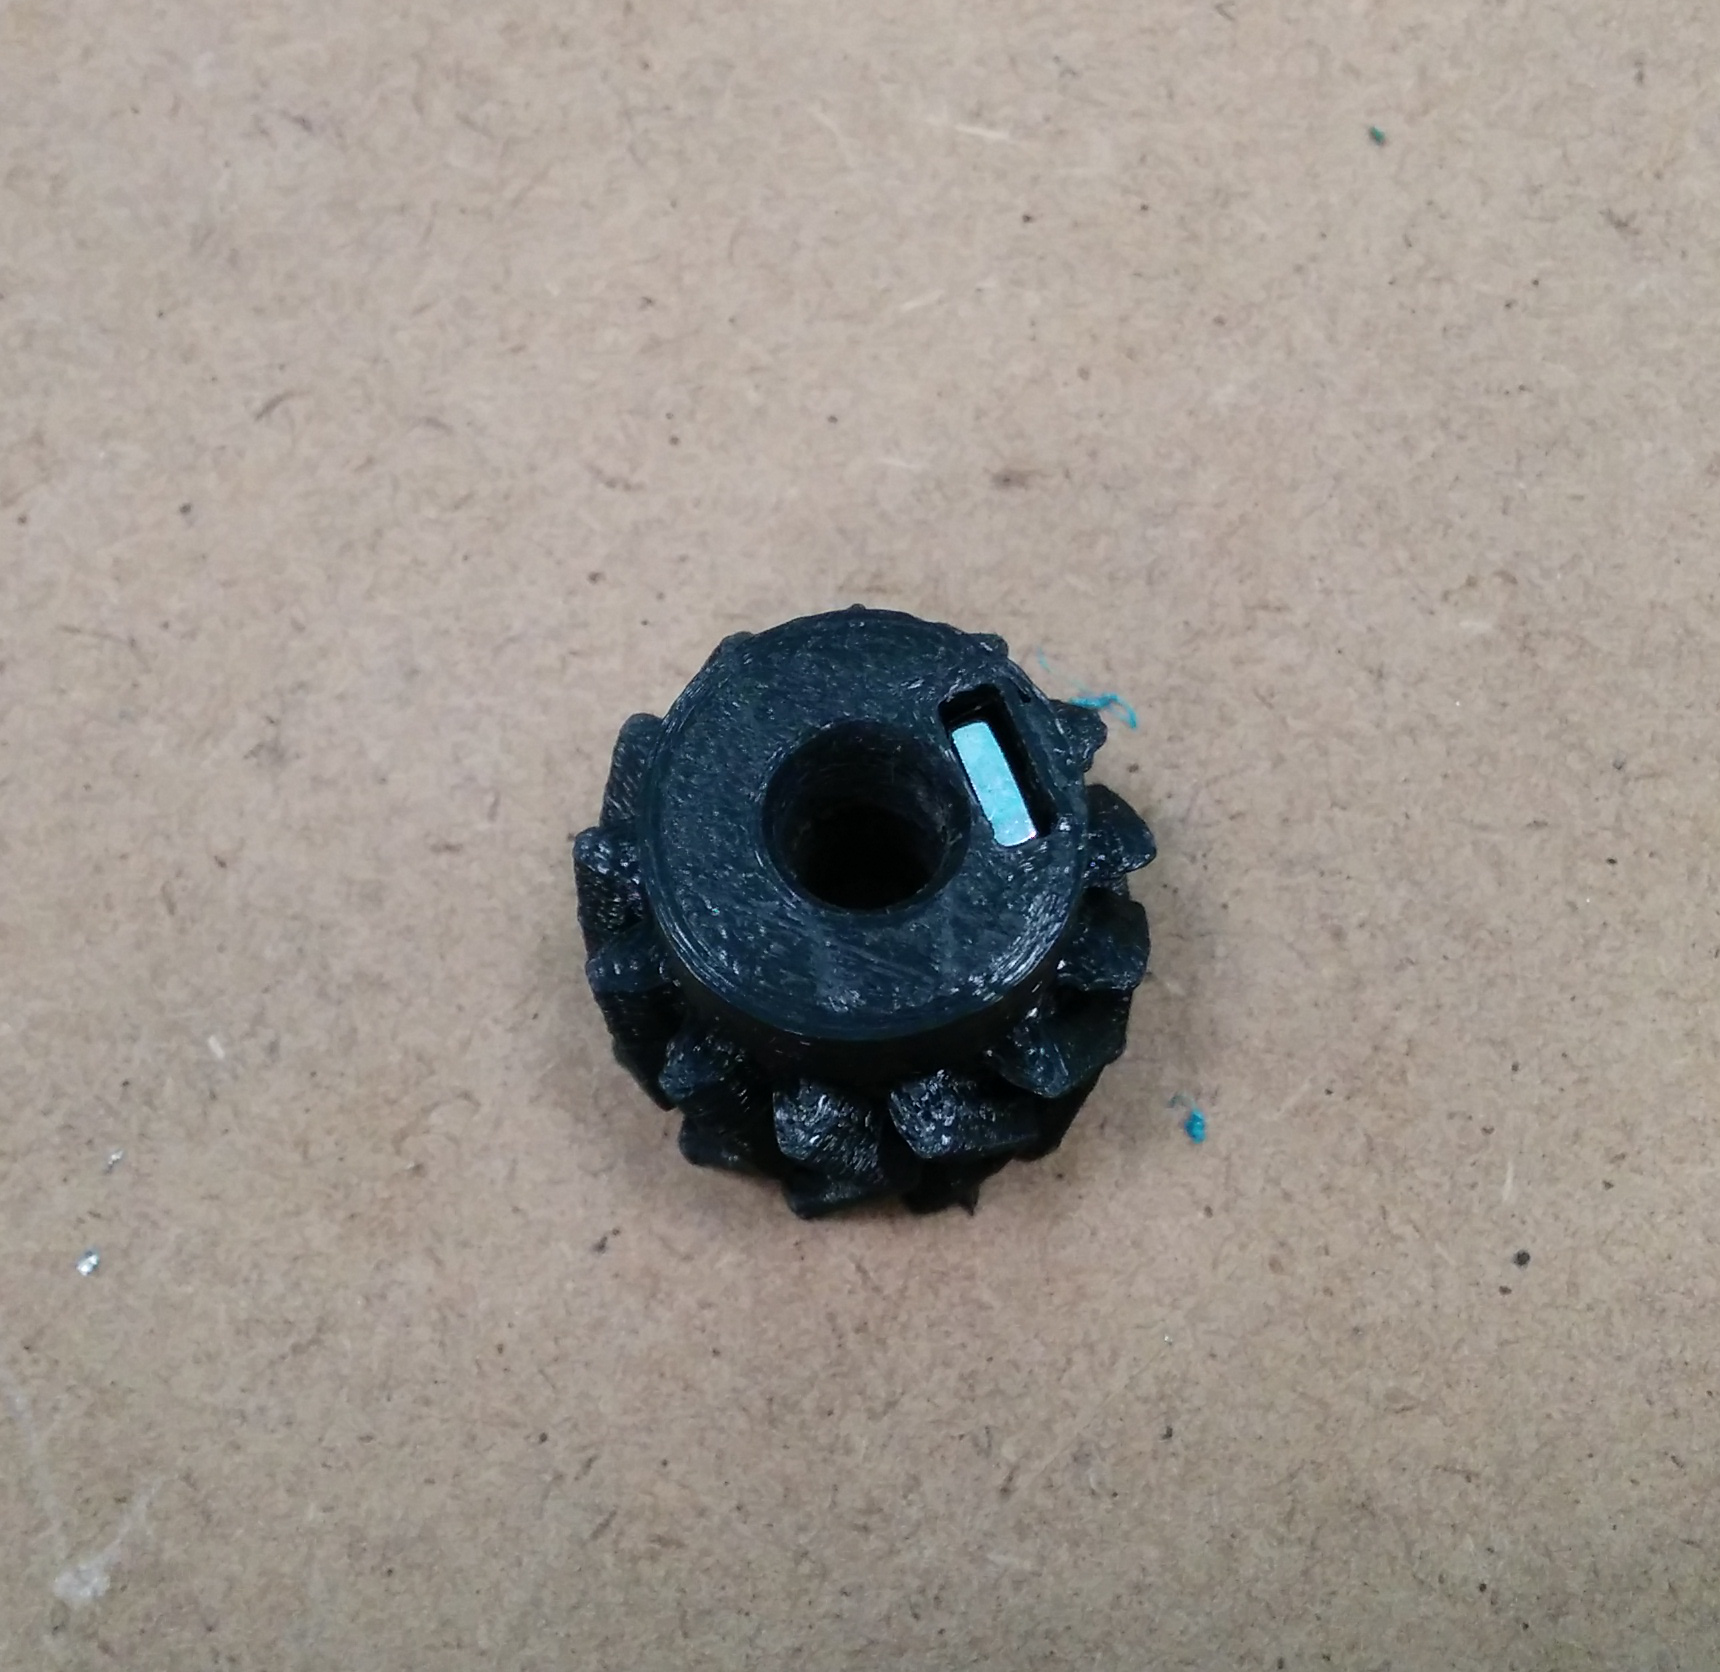
\includegraphics[width=\textwidth]{images/filawinder/montaje2.png}
                \caption{Tuerca en alojamiento de engranaje}
                \label{fig:winder_engranaje}
        \end{subfigure}
        ~
        \begin{subfigure}[b]{0.35\textwidth}
                \centering
                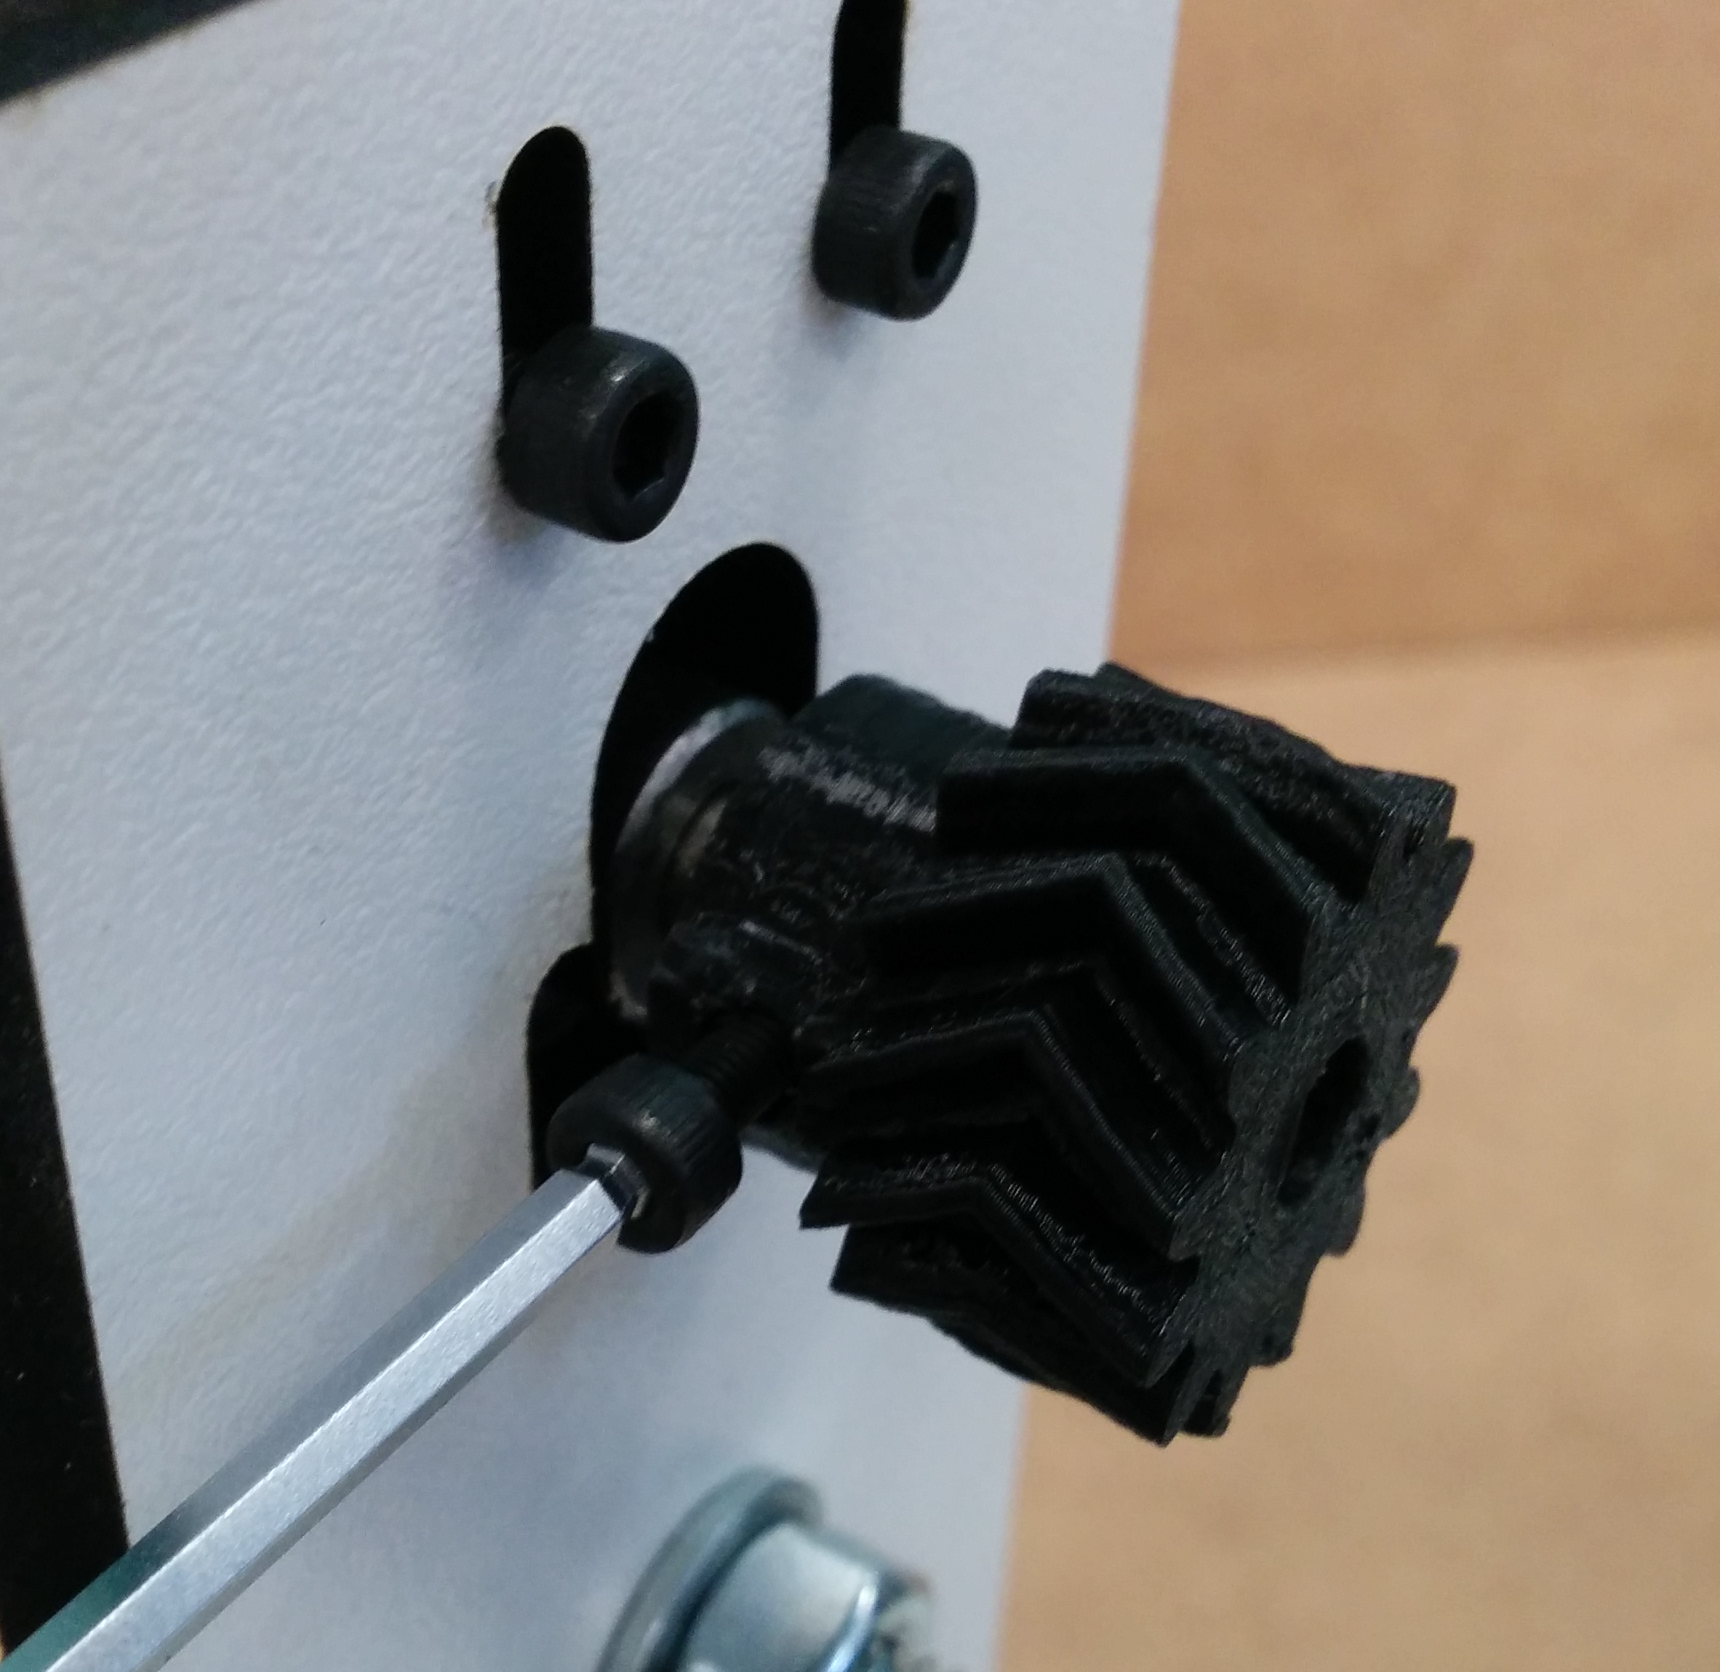
\includegraphics[width=\textwidth]{images/filawinder/montaje3.png}
                \caption{Apriete de engranaje al vástago.}
                \label{fig:winder_apriet}
        \end{subfigure}
        \caption{Montaje del engraneje en eje del motor.}
        \label{fig:winder_montaje_engranaje}
\end{figure}

Situamos la placa electrónica en la parte inferior de la pieza con ayuda de cuatro tornillos M3x12 y cuatro tuercas de M3.

    \begin{figure}[H]
            \centering
            \includegraphics[width=0.5\textwidth]{images/filawinder/montaje4.png}
            \caption{Instalación de la placa electrónica.}
            \label{fig:winder_arduino}
    \end{figure}

Roscamos una tuerca M8 e introducimos una arandela de M8 en la varilla roscada de M8, pasamos la varilla roscada a través del agujero debajo del motor, e introducimos otra arandela y otra tuerca de M8 para apretar el conjunto.

    \begin{figure}[H]
            \centering
            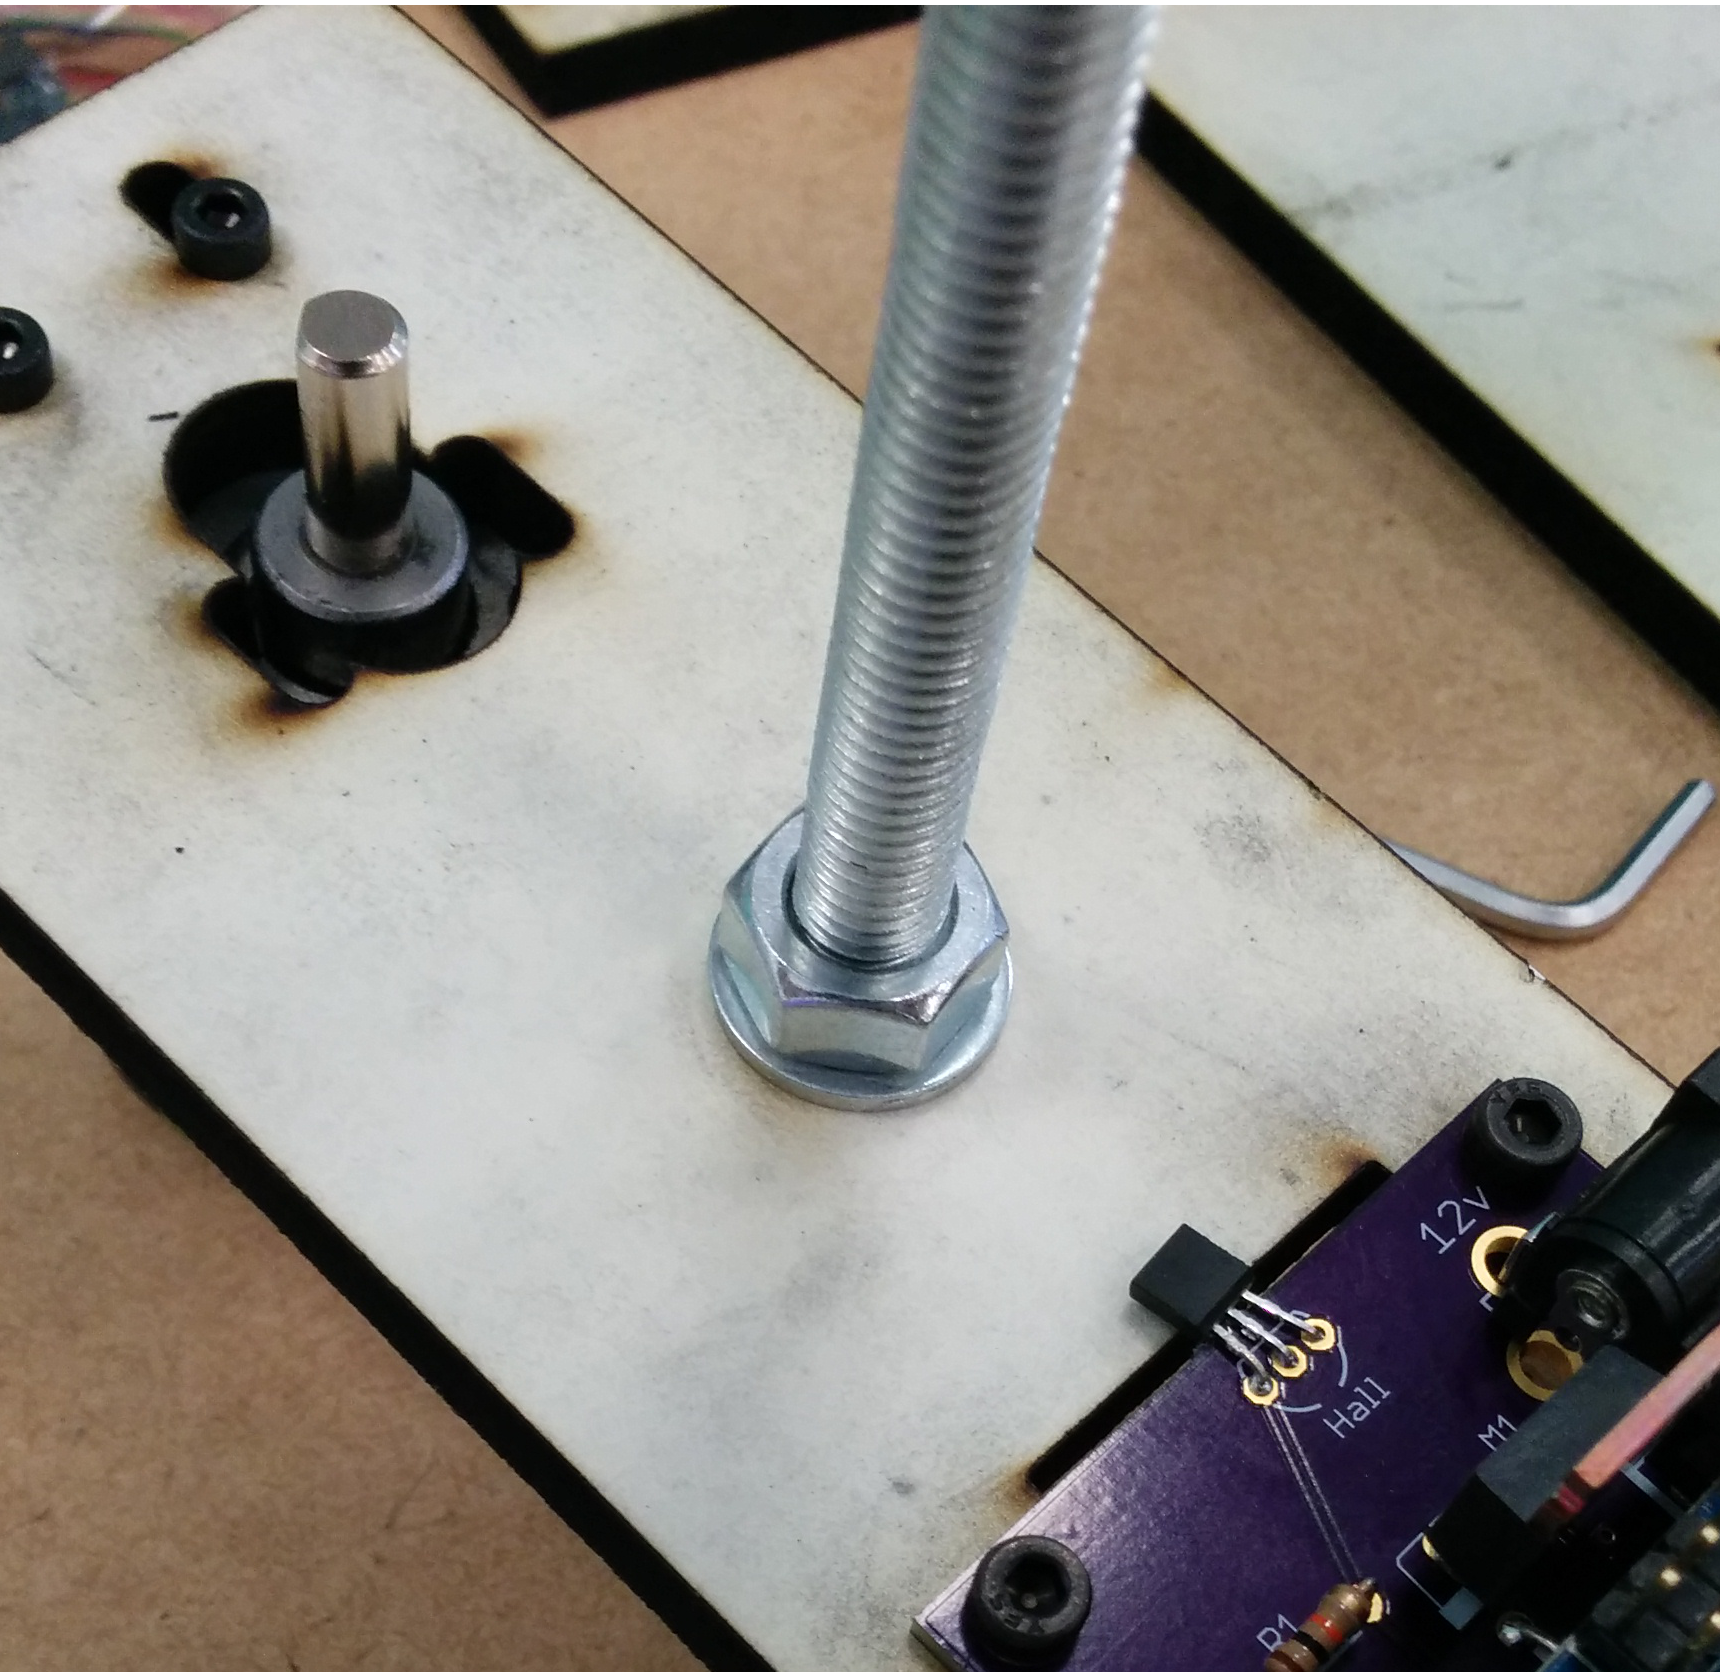
\includegraphics[width=0.5\textwidth]{images/filawinder/montaje5.png}
            \caption{Eje de giro para la bobina.}
            \label{fig:winder_soporte}
    \end{figure}

Alojamos la pieza con el motor, la varilla y la electrónica, en el lateral de la base principal, sujetamos ambas piezas con ayuda de una tuerca y un tornillo de M3x25.

    \begin{figure}[H]
            \centering
            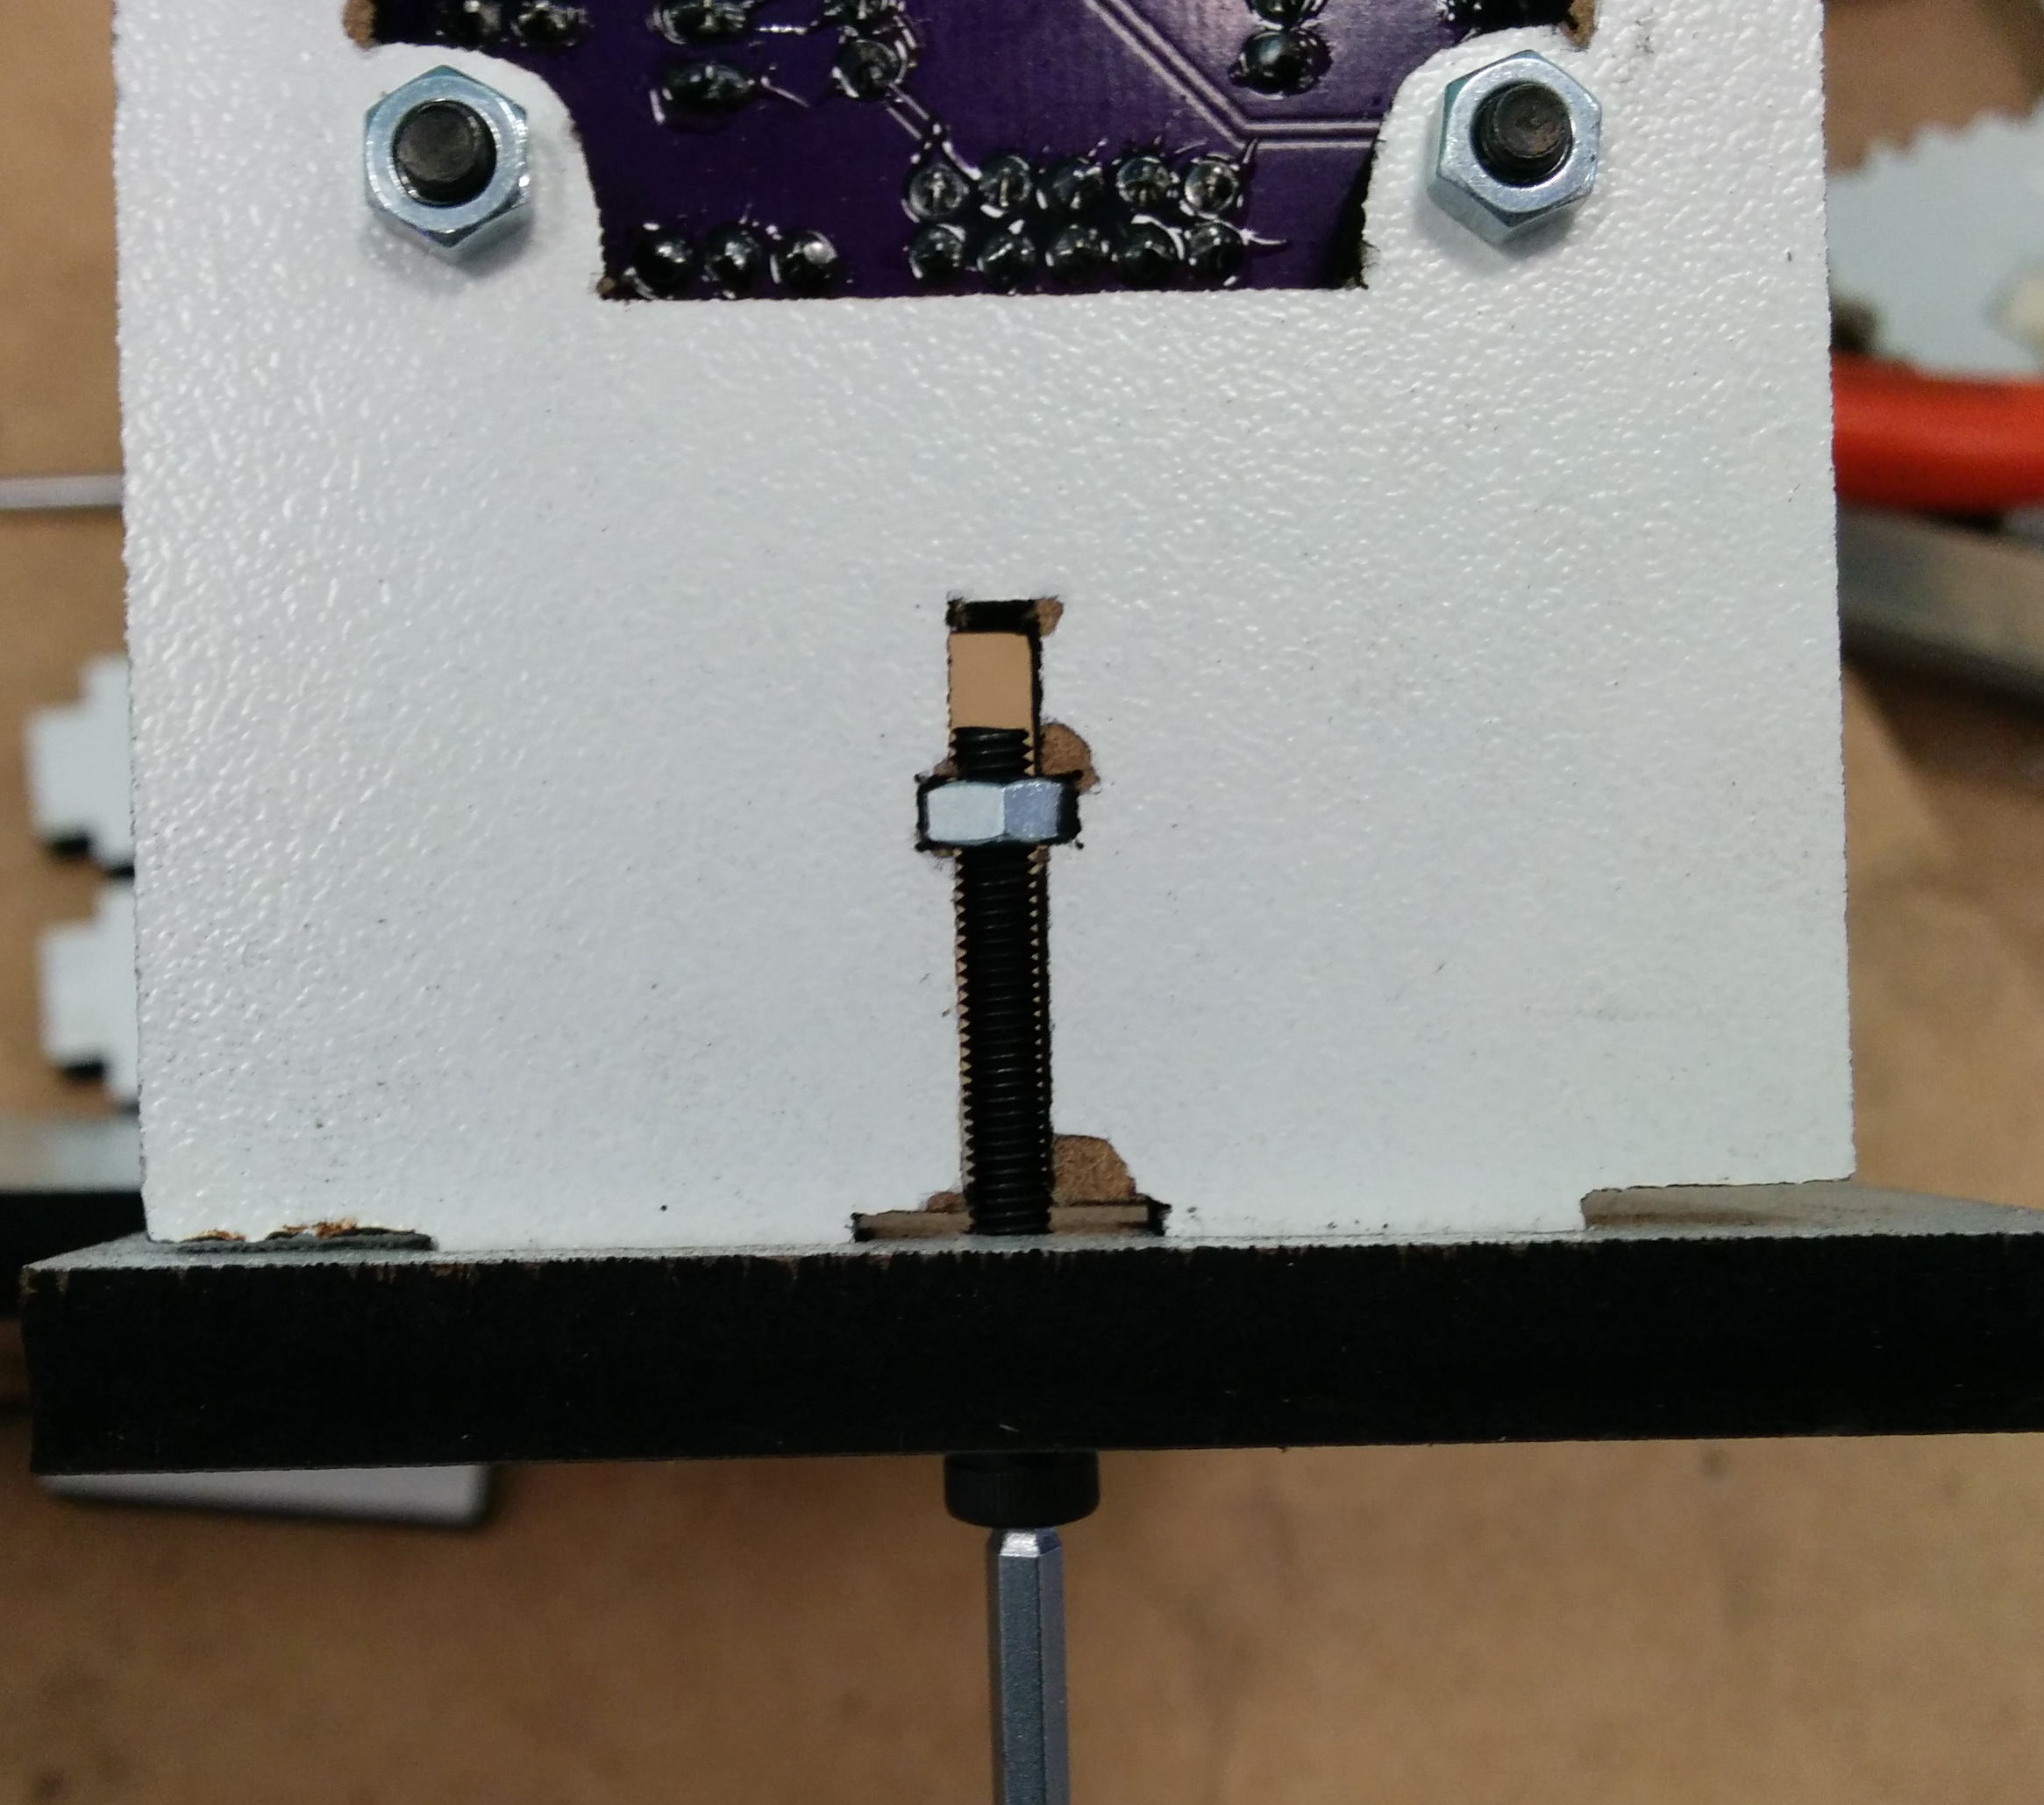
\includegraphics[width=0.5\textwidth]{images/filawinder/montaje6.png}
            \caption{Unión de lateral con base principal.}
            \label{fig:winder_soporte_base}
    \end{figure}


Una vez montada la estructura principal, sérá necesario cablear todos los componentes entre sí. 

    \begin{figure}[H]
          \centering
        \begin{subfigure}[b]{0.35\textwidth}
                \centering
                \includegraphics[width=\textwidth]{images/filawinder/IMG_20150311_123035.jpg}
                \caption{Botonera de control filawinder}
                \label{fig:winder_botonera}
        \end{subfigure}
        ~
        \begin{subfigure}[b]{0.35\textwidth}
                \centering
                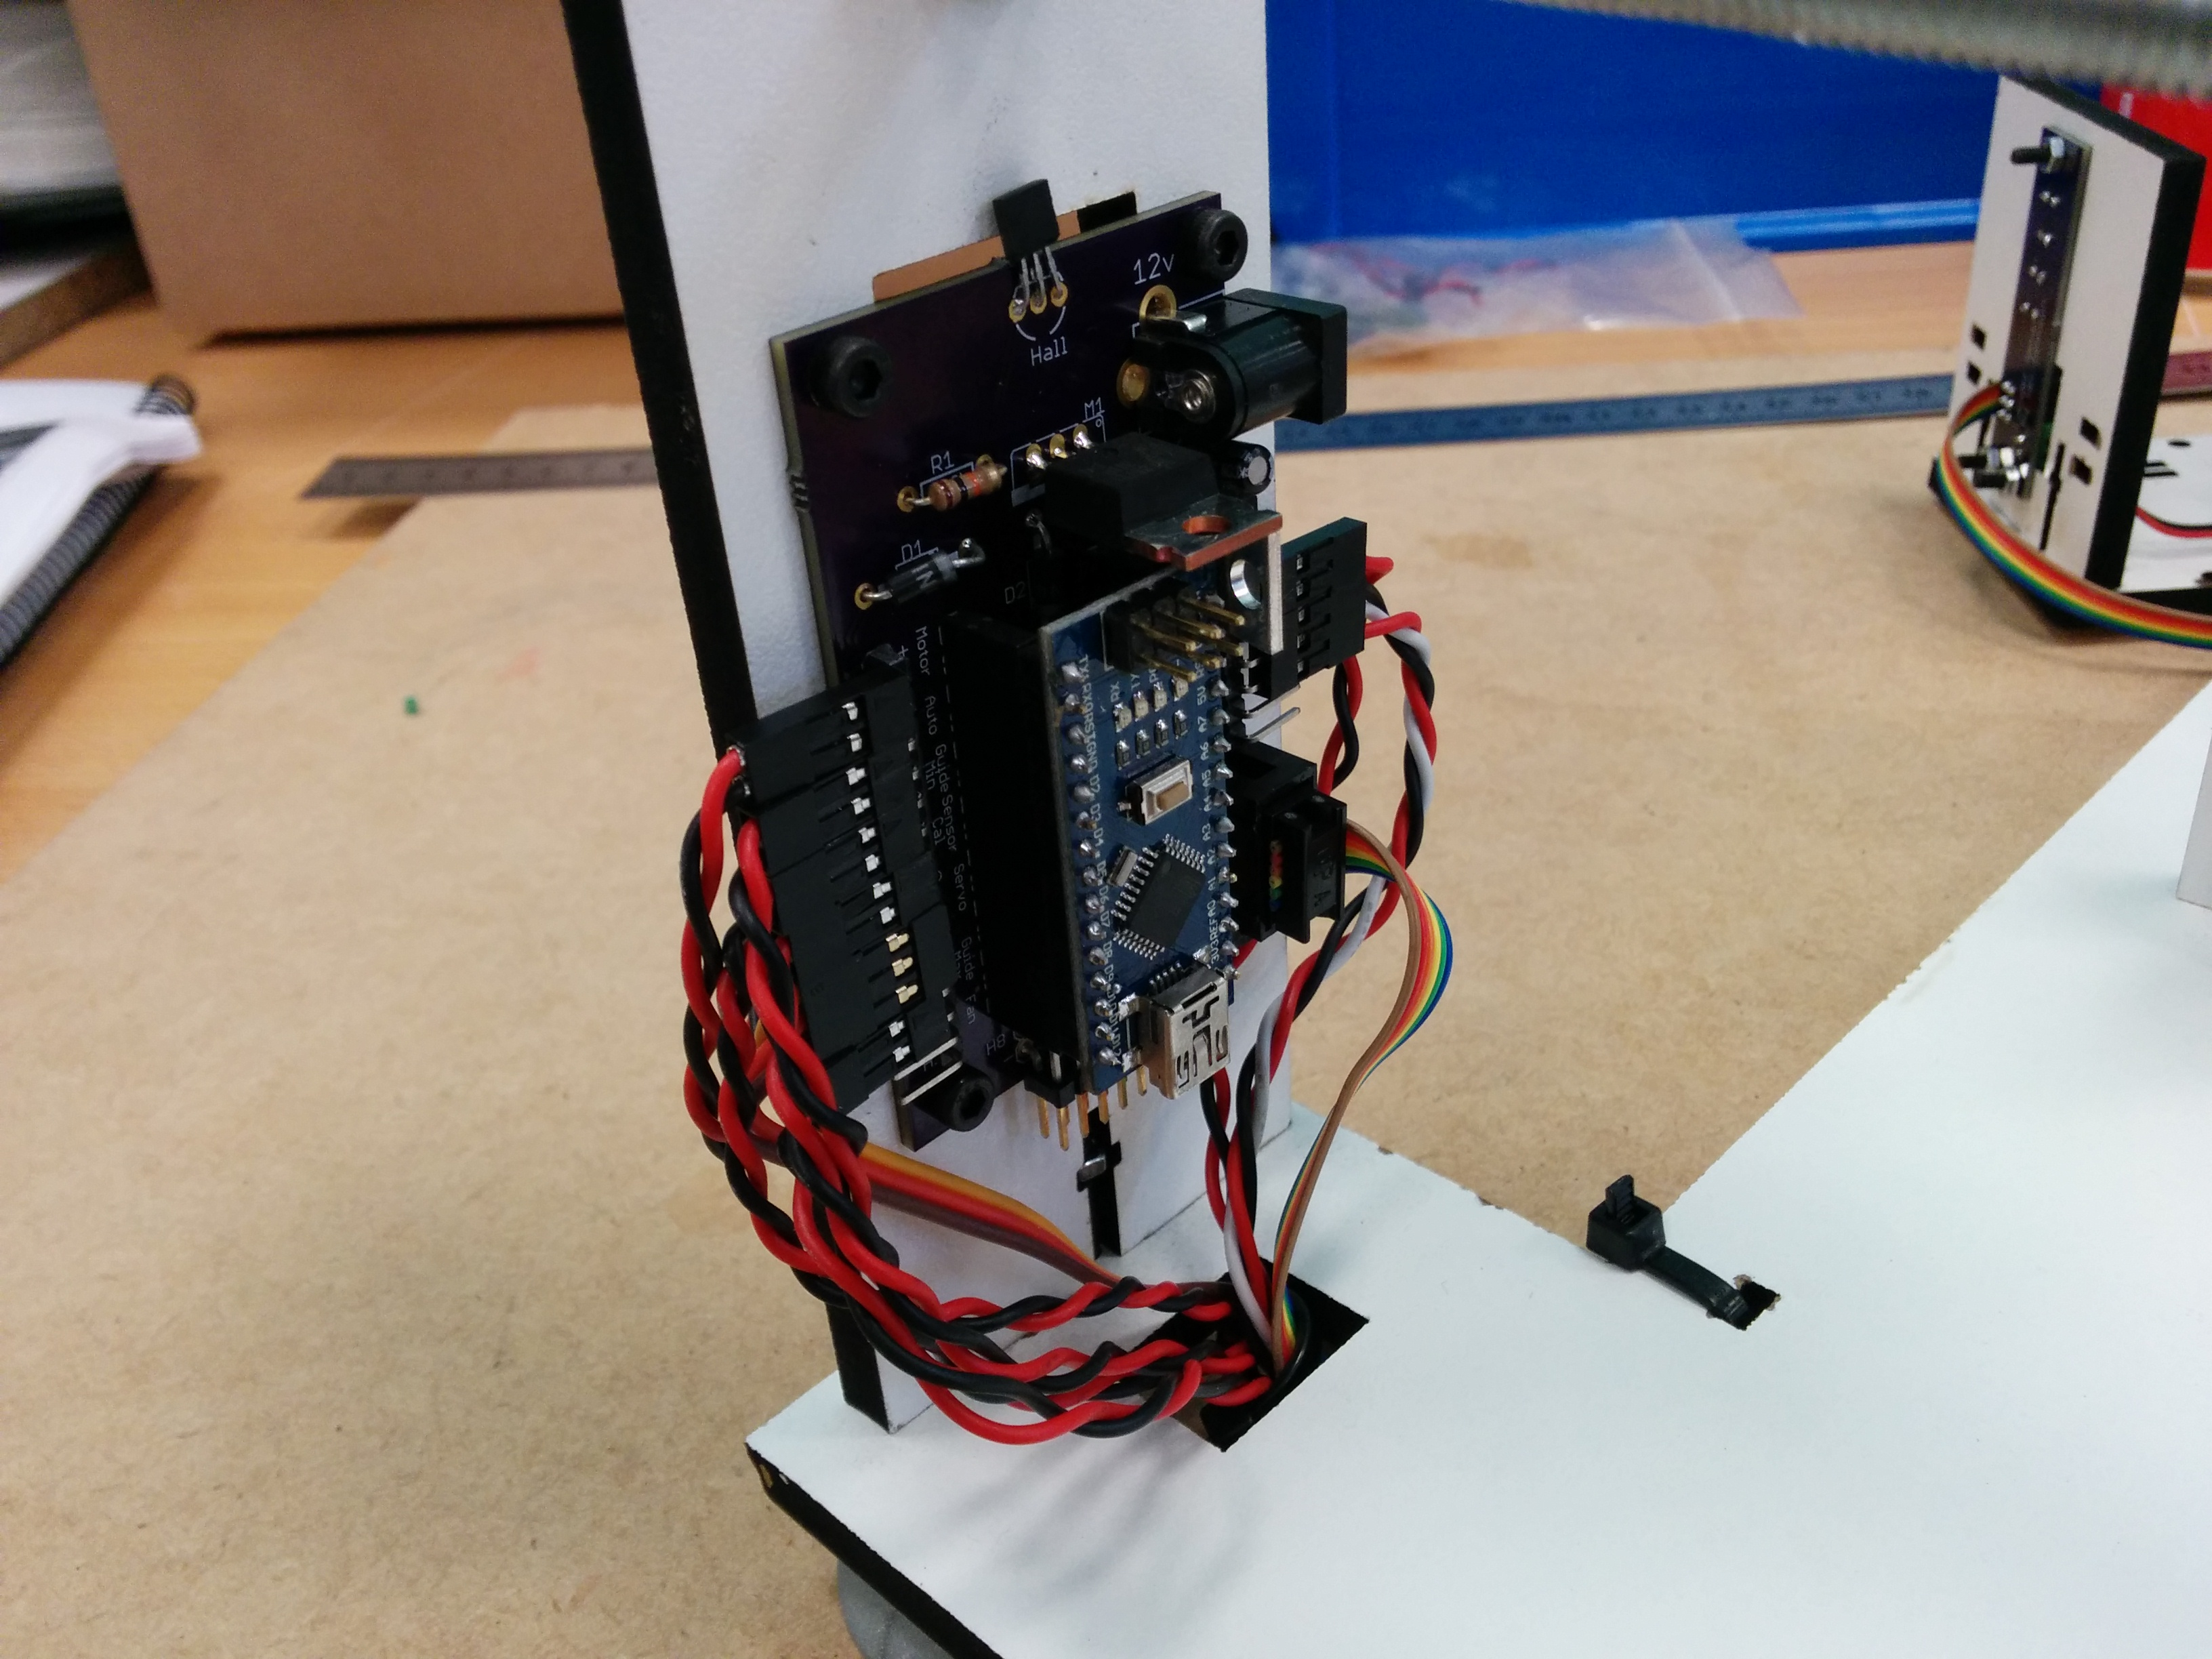
\includegraphics[width=\textwidth]{images/filawinder/IMG_20150311_131828.jpg}
                \caption{Placa controladra cableada.}
                \label{fig:winder_arduino1}
        \end{subfigure}
        \caption{Montaje electrico de la placa de control.}
        \label{fig:winder_montaje_electrio}
\end{figure}

Con esto concluimos el montaje del filawinder, el cual usaremos a la hora de producir filamento.

%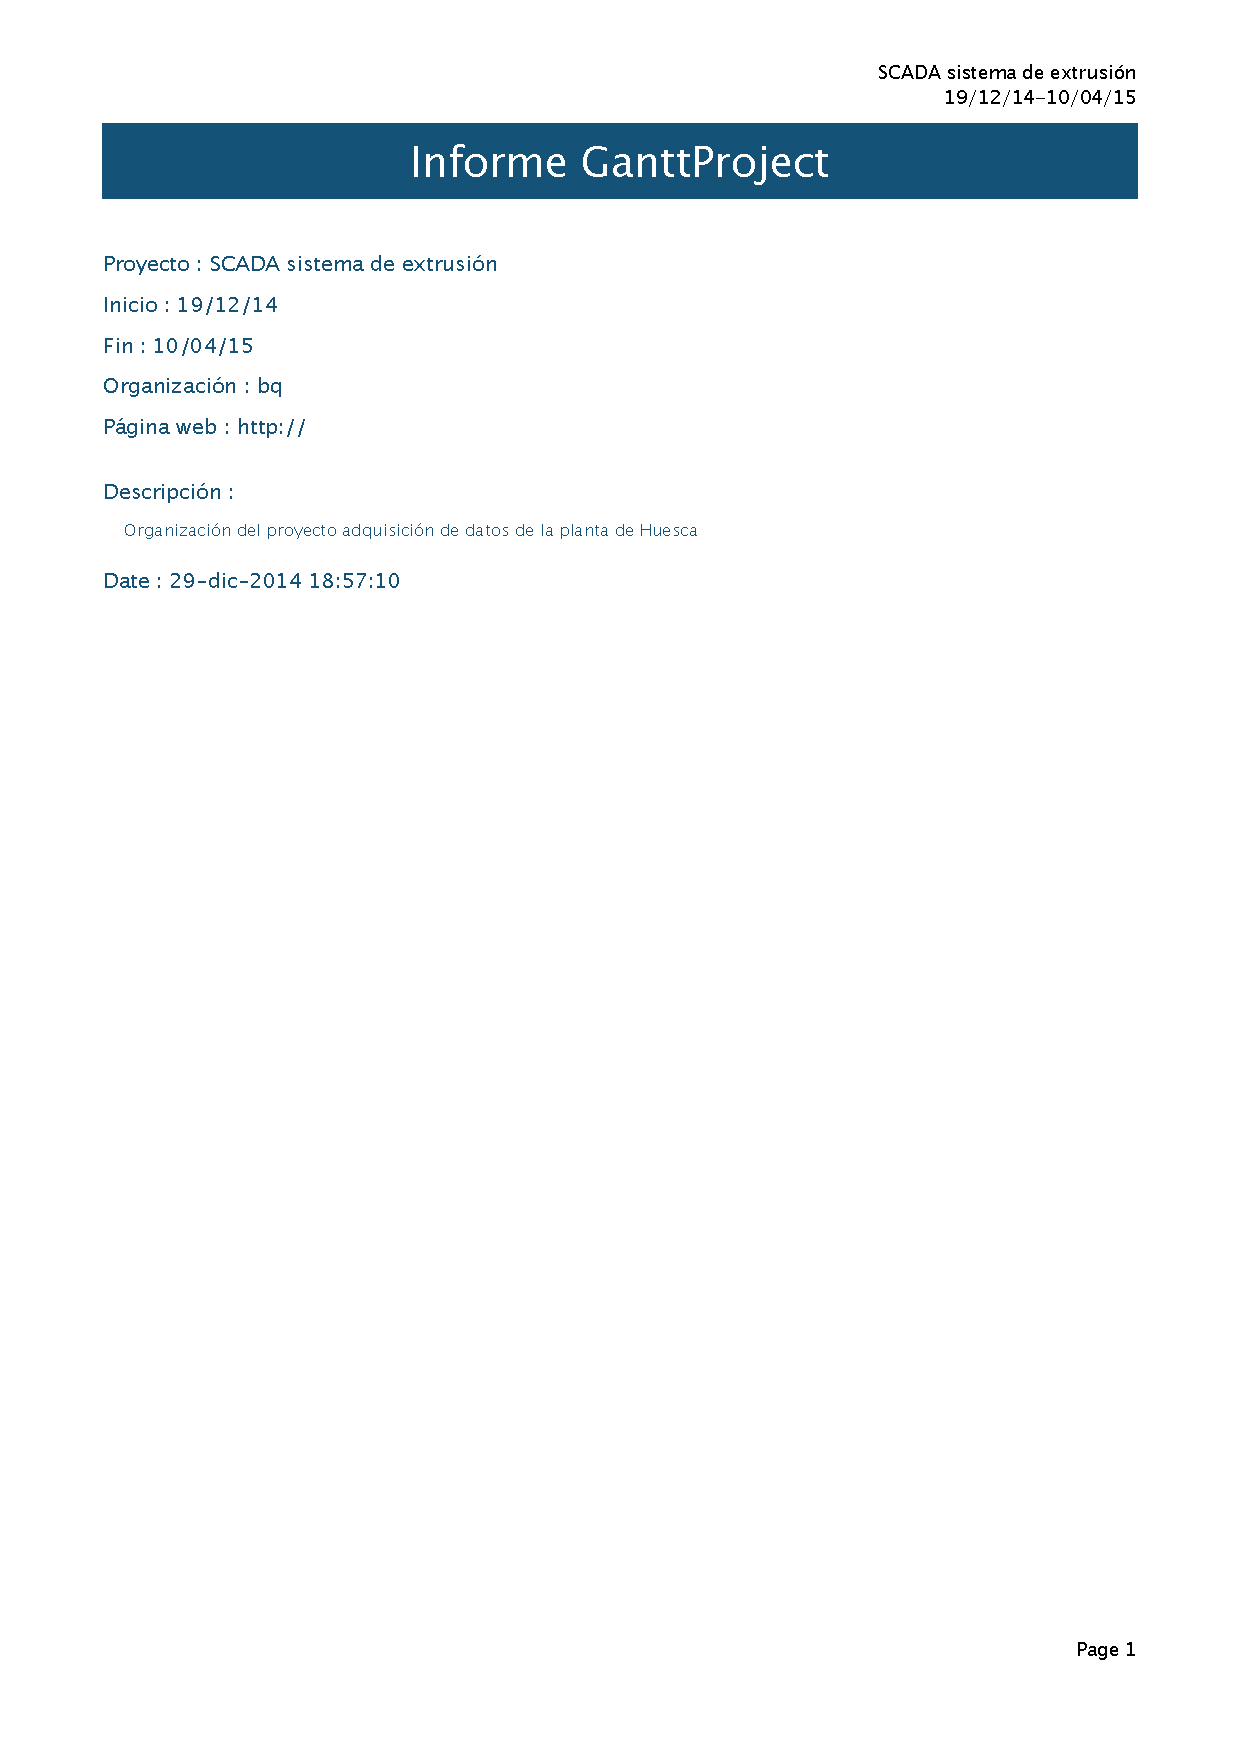
\includepdf[pages=-]{gantt.pdf}

%\chapter{Bibliografia}
\label{bibliografia}
\section{Capítulos}
Cap \ref{arte_extrusion}\\
\url{http://es.wikipedia.org/wiki/Extrusi%C3%B3n}\\
\url{http://es.wikipedia.org/wiki/Extrusi%C3%B3n_de_pol%C3%ADmero}\\
\url{http://elblogdelplastico.blogs.upv.es/2012/10/23/tecnologias-de-fabricacion-con-materiales-polimericos-y-sus-compuestos-3/}\\
\url{http://www.ehu.eus/reviberpol/pdf/NOV13/perez.pdf}\\

\url{http://www.ceautomatica.es/old/actividades/jornadas/XXIX/pdf/264.pdf}\\
\url{http://tv.uvigo.es/uploads/material/Video/1567/ISAD_Tema6.pdf}\\



\url{http://www.stratasys.com/3d-printers/technologies/fdm-technology}\\

\url{https://www.google.com/patents/US5121329}\\

\url{http://www.google.com/patents/US5340433?printsec=abstract#v=onepage&q&f=false}\\
\section{Figuras}
Fig \ref{fig:estado_husillo1}: \url{http://3.bp.blogspot.com/-Z0GzL5mmFW8/TbWU01H0D5I/AAAAAAAAAHE/aW1dNIs0Pl8/s1600/21.JPG}\\
Fig \ref{fig:estado_husillo2}: \url{https://lh4.googleusercontent.com/-38dQ_PeujTE/TYCjbjVFSxI/AAAAAAAAAB8/Ogy3O1i_KCo/s1600/14.JPG}\\
Fig \ref{fig:protocolo_profibus}: \url{http://www.etitudela.com/entrenadorcomunicaciones/downloads/profibusteoria.pdf}

Fig \ref{fig:impr_fdm}: 
\href{http://upload.wikimedia.org/wikipedia/commons/4/42/FDM_by_Zureks.png}{wikimedia}

\newpage{}
\label{Bibliography}
\lhead{\emph{Bibliografia}}  % Change the left side page header to "Bibliography"
\bibliographystyle{unsrt}
\bibliography{references}




\end{document}